\documentclass[11pt]{article}
\usepackage[margin=2.2cm]{geometry}
\usepackage{graphicx,booktabs,amsmath,amssymb,amsthm,enumitem,float,xcolor,caption,microtype,array}
\usepackage{url}
\usepackage[hidelinks]{hyperref}
\usepackage{tikz}
\usetikzlibrary{arrows.meta,positioning,shapes.geometric}
\captionsetup{font=small,labelfont=bf}
\setlist{itemsep=2pt,topsep=4pt}
\newcommand{\kA}{k_A}
\newcommand{\kG}{k_G}
\newcommand{\xc}{x_{0,\mathrm{crit}}}
\newcommand{\zsn}{z_{\mathrm{SN}}}
\newcommand{\xsn}{x_{1,\mathrm{SN}}}
\newcommand{\xh}{x_0^{\mathrm{HSP}}}
\newtheorem*{remark}{Remark}
\definecolor{boxc}{HTML}{F4F3EF}
\newcommand{\keybox}[1]{\par\noindent\colorbox{boxc}{\parbox{\dimexpr\linewidth-2\fboxsep}{\small #1}}\par\medskip}

\title{The Epileptor, and what it means to place a homeostatic-plasticity\\ seizure cycle in its coordinates}
\author{}
\date{Working notes, version 2: single-gain mapping and the equation for $x_0(t)$\\ (version 1: \texttt{report\_v1.pdf})}

\begin{document}
\maketitle
\tableofcontents
\newpage

%==========================================================================================
\section{Why connect the two models}
%==========================================================================================
Our spiking E/I network with homeostatic synaptic plasticity (HSP) produces cycles of seizure risk
\emph{mechanistically}. Under a reduced drive (36\,Hz instead of 40\,Hz: deafferentation), HSP slowly raises recurrent
excitation ($\kA\uparrow$) and lowers inhibition ($\kG\downarrow$) until the network ignites into a high-rate state. The
over-activity then makes HSP remove excitation, which ends the high-rate state and leaves a long quiet period. The cycle
repeats on its own. Its time scale is set by the HSP time constants, which are compressed in the model (minutes to hours,
to simulate many cycles) but are thought to be days in the brain. With realistic constants, each high-rate state is a
\emph{high-risk period} lasting days, and each quiet period a \emph{low-risk period} lasting weeks, as in the multidien
cycles seen in patients.

The \emph{Epileptor} \cite{jirsa2014} is the opposite kind of model: phenomenological, a handful of differential
equations built to reproduce the \emph{dynamical signature} of seizures (how they start, how they end, how they recur),
without committing to a biophysical mechanism. Its excitability $x_0$ is what the Virtual Epileptic Patient pipeline
infers for each brain region \cite{jirsa2017,proix2017}, and it is the model of seizures in The Virtual Brain (TVB)
\cite{sanzleon2013}.

The goal of this report is practical:
\keybox{\textbf{Write the Epileptor's excitability as a slowly varying $x_0(t)$ that follows the HSP equations, in the
simplest form that is still correct, so that it can later be used in TVB (different deafferentations in different brain
regions, coupled through the connectome).}}
Here the mapping is \emph{post hoc}: nothing is fed back into the spiking network. We re-express its recorded HSP state as
$x_0(t)$, check that the Epileptor geometry organises it, and derive the equation that $x_0$ itself obeys.

%==========================================================================================
\section{The Epileptor}
%==========================================================================================
\subsection{Where it comes from: a bifurcation taxonomy of seizures}
Jirsa et al. \cite{jirsa2014} started from a dynamical-systems observation. A seizure is a transition between
two states of a neural population, a resting (interictal) state and an oscillatory (ictal) state, and such
transitions are \emph{bifurcations} of a fast subsystem driven by a slower variable. The kind of bifurcation leaves
fingerprints in the recordings:
\begin{itemize}
\item \textbf{Onset by a saddle-node bifurcation}: a rest state and a saddle collide and disappear; the system jumps to
an oscillation whose amplitude is finite immediately and whose baseline shifts. This matches the \emph{DC shift}
often seen at seizure onset.
\item \textbf{Offset by a homoclinic bifurcation}: the oscillation ends when the limit cycle collides with a saddle;
the inter-spike interval grows logarithmically as the bifurcation is approached, i.e. the discharge
\emph{slows down} before stopping, while the amplitude stays roughly constant. This matches the
frequency-slowing at the end of many focal seizures.
\end{itemize}
A fast subsystem that is pushed back and forth through a saddle-node (onset) and a homoclinic (offset) bifurcation
by a slow variable is a \emph{square-wave burster} in Izhikevich's classification of bursters \cite{izhikevich2000}.
The Epileptor is the minimal model of that class with the additional ingredients needed to reproduce human and animal
seizure recordings. Later work generalised the idea to a full taxonomy of 16 onset/offset ``dynamotypes'', among which
the Epileptor's saddle-node/homoclinic pair is one of the most frequently observed in patient recordings \cite{saggio2020}.

\subsection{The full model (five state variables plus a filter)}
With TVB's default parameters \cite{sanzleon2013}:
\begin{align}
\dot x_1 &= y_1 - f_1(x_1, x_2, z) - z + I_{ext,1}, &
\dot y_1 &= c - d\,x_1^2 - y_1, \label{eq:pop1}\\
\dot z   &= r\,\big[\,s\,(x_1 - x_0) - z - 0.1\,z^7\,\mathbf 1_{z<0}\big], \label{eq:z}\\
\dot x_2 &= -y_2 + x_2 - x_2^3 + I_{ext,2} + b_2\, g - 0.3\,(z - 3.5), &
\dot y_2 &= \tfrac{1}{\tau_2}\,\big(-y_2 + f_2(x_2)\big), \label{eq:pop2}\\
\dot g &= -0.01\,(g - 0.1\,x_1), \label{eq:g}
\end{align}
with
\[
f_1 = \begin{cases} a x_1^3 - b x_1^2, & x_1 < 0\\ -\big(\mathrm{slope} - x_2 + 0.6\,(z-4)^2\big)\,x_1, & x_1\ge 0\end{cases}
\qquad
f_2 = \begin{cases} 0, & x_2 < -0.25\\ a_2\,(x_2 + 0.25), & x_2 \ge -0.25.\end{cases}
\]
Parameters: $a=1$, $b=3$, $c=1$, $d=5$, $s=4$, $I_{ext,1}=3.1$, $I_{ext,2}=0.45$, $\tau_2=10$, $a_2=6$,
$b_2=2$, slope $=0$, $r=0.00035$, and $x_0$ (TVB default $-1.6$; the critical value is near $-2.06$, see below).

\begin{table}[H]\centering\small
\begin{tabular}{>{\raggedright}p{2.7cm}>{\raggedright}p{3.3cm}p{8.6cm}}
\toprule
variables & name & role \\
\midrule
$(x_1, y_1)$ & population 1 & fast discharges; its bistability (rest vs oscillation) creates onset and offset \\
$(x_2, y_2)$ & population 2 & slower spike-and-wave events ($\tau_2=10$) superimposed during the seizure \\
$g$ & low-pass coupling & population 1 drives population 2 through a slow filter of $x_1$ \\
$z$ & \emph{permittivity} (slow) & time scale $1/r \approx 2857$ units; integrates $x_1$ and moves population 1 across its bifurcations \\
$x_0$ & excitability (parameter) & position of the slow nullcline; decides whether a stable rest state exists \\
\bottomrule
\end{tabular}
\caption{The Epileptor's subsystems.}
\end{table}

\textbf{How a seizure unfolds} (Fig.~\ref{fig:6d}). Between seizures, $x_1$ sits at a rest state on the left
branch of population 1's nullcline, and $z$ slowly \emph{decreases} (because $s(x_1 - x_0) < z$ there). When $z$ falls
below the saddle-node value, the rest state disappears: $x_1$ jumps to the oscillatory branch (onset: DC shift and fast
discharges), population 2 starts producing spike-wave events, and $z$ now \emph{increases}, since $x_1$ is high. Rising
$z$ moves population 1 towards the homoclinic bifurcation, the discharges slow down and stop (offset), and $x_1$ falls
back to rest, where $z$ decreases again. The seizure is thus a hysteresis loop of the fast subsystem, driven by $z$.
$z$ is a \emph{negative feedback} that accumulates during the seizure and terminates it; it has been interpreted as a
slow process such as changes in extracellular ion concentrations or energy metabolism, but the model does not depend
on that interpretation \cite{jirsa2014}.

\begin{figure}[H]\centering
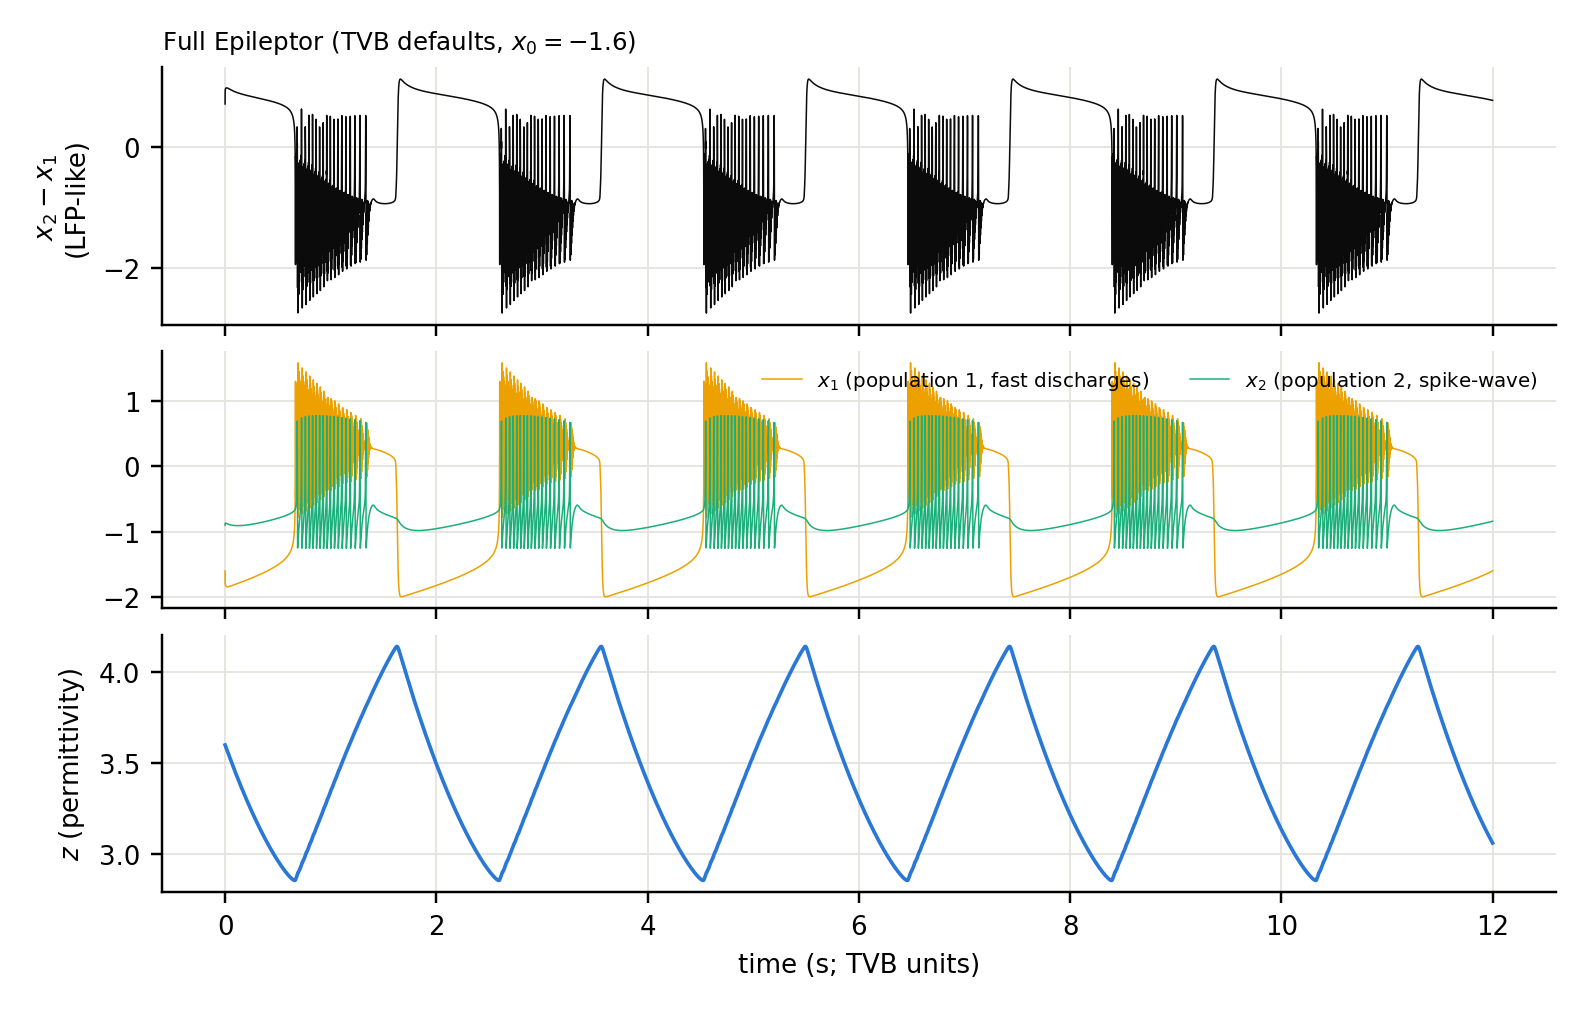
\includegraphics[width=0.95\linewidth]{figs/th_6d.png}
\caption{The full Epileptor with TVB defaults ($x_0=-1.6$, supercritical), integrated with LSODA. Top: the LFP-like
signal $x_2 - x_1$, with the DC shift at onset, fast discharges and spike-wave complexes. Middle: the two populations.
Bottom: $z$ is a sawtooth: it falls between seizures and rises during them. In TVB units (1 unit $=$ 1\,ms) a
seizure lasts $\sim0.7$\,s; in practice the time axis is rescaled to the data.}\label{fig:6d}
\end{figure}

\textbf{Time units.} The Epileptor equations have no intrinsic time unit. TVB integrates them with the step in
milliseconds and $r=0.00035$, i.e.\ $1/r\approx2.9$\,s. Seizure duration and recurrence scale with $1/r$ and with
$x_0$, so when fitting data the time axis (or $r$) is usually rescaled. This matters for us (Section~\ref{sec:timescales}).

\subsection{The excitability $x_0$ and the slow nullcline}
$x_0$ appears only in the $z$ equation \eqref{eq:z}. Setting $\dot z=0$ gives the \emph{slow nullcline}
$z = s(x_1 - x_0)$, a straight line of slope $s=4$; increasing $x_0$ shifts it to the right (or down). The rest state
is the intersection of this line with the left (interictal) branch of the fast nullcline. If the line intersects
the branch to the left of its fold, the intersection is a stable fixed point and the region rests indefinitely
(\emph{subcritical}). If $x_0$ is large enough that the line passes the fold, there is no stable rest state on that
branch, and the region seizes periodically on its own (\emph{supercritical}). This is why, in the Virtual Epileptic
Patient, $x_0$ is the quantity that labels a region as epileptogenic (above the critical value), as part of the
propagation zone (close below it, so that input from other regions can push it over), or healthy (far below)
\cite{jirsa2017,proix2017}.

\subsection{The 2D reduction used here}
Proix et al. \cite{proix2014} reduced the Epileptor to two variables to study seizure propagation across regions.
Two steps:
\begin{enumerate}
\item $y_1$ is fast compared with $z$; on the interictal branch it relaxes to $y_1 = c - d x_1^2 = 1 - 5x_1^2$.
\item Population 2 and the filter are dropped (they shape the ictal waveform, not the onset).
\end{enumerate}
Substituting $y_1$ and the $x_1<0$ form of $f_1$ into \eqref{eq:pop1}:
\[
\dot x_1 = (1 - 5x_1^2) - (x_1^3 - 3x_1^2) - z + I_{ext}
        = -x_1^3 - 2x_1^2 + 1 - z + I_{ext},
\]
\begin{equation}\boxed{\;\dot x_1 = -x_1^3 - 2x_1^2 + 1 - z + I_{ext}, \qquad
\dot z = r\left[\,4(x_1 - x_0) - z - 0.1\,z^7\mathbf 1_{z<0}\right]\;}\label{eq:2d}\end{equation}
($I_{ext}=3.1$, $r=0.00035$; in network versions a coupling term is added to $\dot z$, the ``permittivity coupling'' by
which a seizing region recruits its neighbours \cite{proix2014}; we have a single region and no coupling).
The fast equation is now a cubic for all $x_1$. Its upper branch replaces the oscillatory branch of the full model:
the 2D reduction keeps the \emph{onset} geometry exactly, but the homoclinic offset becomes a second fold (end of the
upper branch) and the ictal fast oscillations are averaged out.

\subsection{The fold and the critical excitability}\label{sec:fold}
Write the fast nullcline ($\dot x_1=0$) as $z = G(x_1) := -x_1^3 - 2x_1^2 + 1 + I_{ext}$. Its turning points satisfy
\[
G'(x_1) = -3x_1^2 - 4x_1 = 0 \quad\Rightarrow\quad x_1 = 0 \ \ \text{or}\ \ x_1 = \xsn = -\tfrac43 .
\]
$G''(-4/3) = -6(-4/3) - 4 = 4 > 0$: $x_1=-4/3$ is a local minimum of $G$, the lower end (fold) of the interictal
branch $x_1 < -4/3$; $x_1 = 0$ is a local maximum, the upper end of the ictal branch $x_1>0$. The fold value is
\[
\zsn = G(-\tfrac43) = \tfrac{64}{27} - \tfrac{32}{9} + 1 + I_{ext} = I_{ext} - \tfrac{5}{27} = 2.91481,
\qquad G(0) = 1 + I_{ext} = 4.1 .
\]
For fixed $z$, the fast subsystem has an interictal rest state only if $z \ge \zsn$ (the lower root of $G(x_1)=z$
exists), and an ictal state only if $z \le 4.1$. The slow nullcline passes through the fold when
$\zsn = 4(\xsn - x_0)$:
\begin{equation}\boxed{\;\xc = \xsn - \frac{\zsn}{4} = -\frac43 - \frac{I_{ext} - 5/27}{4} = -2.06204\;}\label{eq:xc}\end{equation}

\textbf{Stability (a subtlety).} With slope 4, the slow nullcline crosses the cubic exactly once, for every $x_0$
(Fig.~\ref{fig:bif}): the 2D system has a \emph{single} fixed point $(x_1^*, z^*)$, which never disappears. Its
Jacobian is
\[
J = \begin{pmatrix} G'(x_1^*) & -1 \\ 4r & -r\end{pmatrix},\qquad
\det J = r\,\big(3x_1^{*2} + 4x_1^* + 4\big) > 0,\qquad \operatorname{tr} J = G'(x_1^*) - r .
\]
The determinant is always positive (the quadratic has no real root), so there is no saddle-node of the full system.
Stability is lost when the trace changes sign, $G'(x_1^*) = r$, i.e.\ when the fixed point moves past the fold onto the
middle (repelling) branch: a Hopf bifurcation at $x_1^* \approx -4/3 + r/4$, which is within $O(r)\sim10^{-4}$ of $\xc$.
Because $r$ is tiny, this Hopf is \emph{singular}: the cycle born there explodes, over an exponentially small range of
$x_0$, into the large relaxation oscillation (a canard explosion \cite{krupa2001,kuehn2015}). So the ``saddle-node''
in the Epileptor's description refers to the \emph{fast} subsystem ($x_1$ at fixed $z$), whose rest state collides
with a saddle at $z=\zsn$; the full 2D system switches from rest to seizures at $x_0 \approx \xc$ through the
fixed point crossing that fold. In the limit $r\to0$ the two pictures coincide, and $\xc$ is the onset threshold.

\begin{figure}[H]\centering
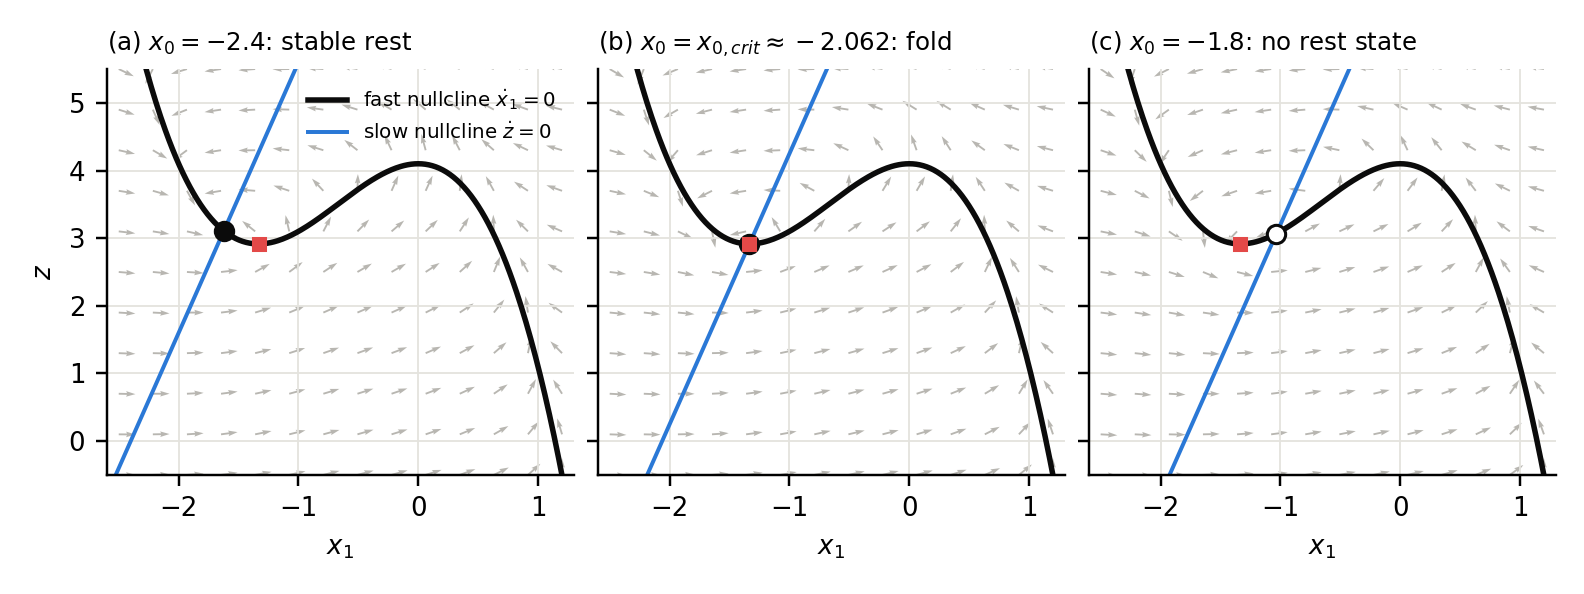
\includegraphics[width=\linewidth]{figs/th_phase_planes.png}
\caption{Phase planes of the 2D Epileptor. Black: fast nullcline $z = G(x_1)$; blue: slow nullcline
$z = 4(x_1 - x_0)$; red square: the fold $(\xsn, \zsn)$; filled/open circle: stable/unstable fixed point; grey arrows:
direction of the flow (slow component exaggerated 400$\times$). (a) Subcritical: the rest state is on the interictal
branch. (b) Critical: the slow nullcline passes through the fold. (c) Supercritical: the only fixed point is on the
repelling middle branch, so the system oscillates.}\label{fig:phase}
\end{figure}

\begin{figure}[H]\centering
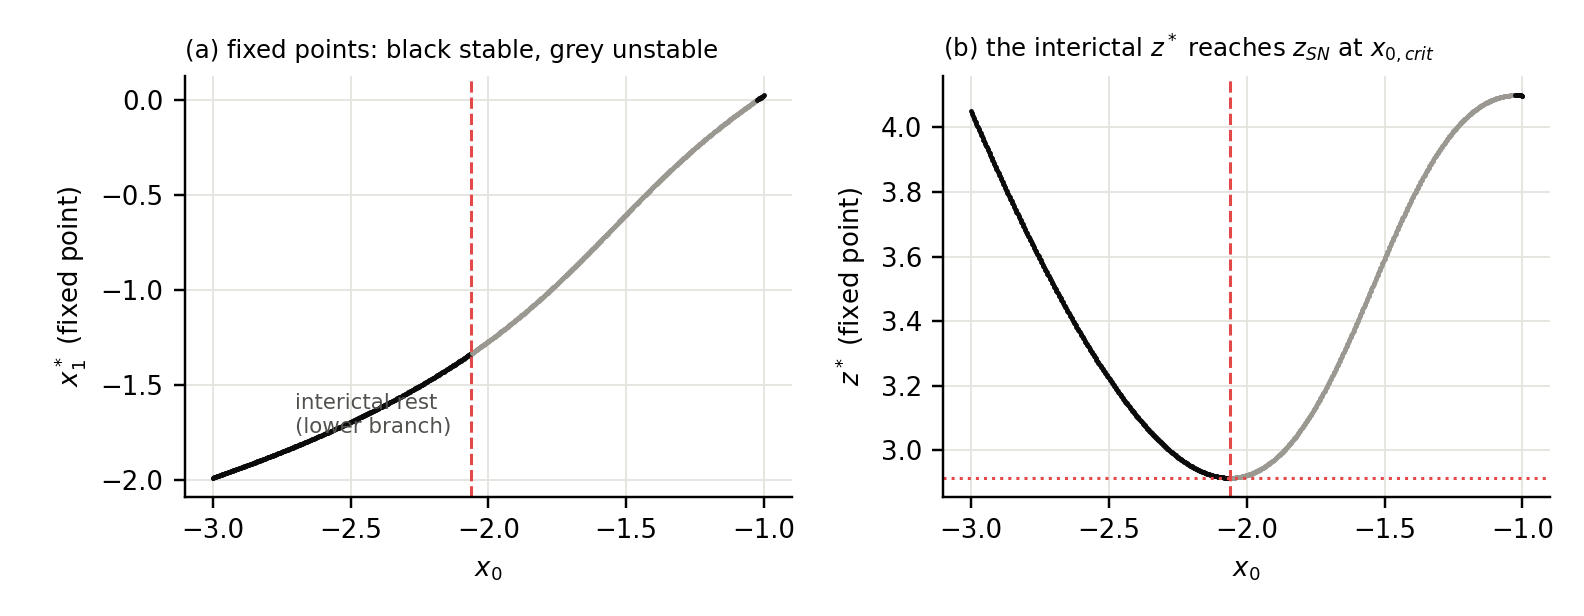
\includegraphics[width=\linewidth]{figs/th_bifurcation.png}
\caption{Fixed point of the 2D Epileptor against $x_0$. It is unique and moves continuously; it is stable (black) on
the interictal branch and loses stability at $\xc$ (red dashed). (b) At $\xc$, $z^*$ reaches its minimum $\zsn$
(dotted).}\label{fig:bif}
\end{figure}

\subsection{Reading the phase plane, step by step}\label{sec:pp}
Figures~\ref{fig:phase} and~\ref{fig:bif} summarise the geometry in one picture each. This section takes them apart: what
each arrow means, why one branch attracts and another repels, why panel (c) of Fig.~\ref{fig:phase} has no stable rest
state although its arrows look almost the same as in (a), and what happens to the fixed point as $x_0$ increases.

\subsubsection*{Step 1: the arrows are the velocity}
At every point $(x_1, z)$ the system moves with velocity
\[
(\dot x_1,\ \dot z) = \big(\,G(x_1) - z,\ \ r\,[4(x_1 - x_0) - z]\,\big),\qquad G(x_1) = -x_1^3 - 2x_1^2 + 1 + I_{ext}.
\]
Each component has a sign that changes on one nullcline:
\begin{itemize}
\item $\dot x_1>0$ (arrow to the \textbf{right}) \textbf{below} the fast nullcline $z = G(x_1)$; $\dot x_1<0$ (left)
above it; vertical arrows on it.
\item $\dot z>0$ (arrow \textbf{up}) \textbf{below} the slow nullcline $z = 4(x_1 - x_0)$, i.e.\ to its lower right;
$\dot z<0$ (down) above it, to its upper left; horizontal arrows on it.
\end{itemize}
The two curves cut the plane into four regions (right--up, right--down, left--up, left--down). Their sizes differ
enormously: $|\dot x_1|$ is of order 1 while $|\dot z|$ carries the factor $r = 0.00035$, so away from the fast
nullcline every true arrow is horizontal (the figures multiply $\dot z$ by 400 so that its sign is visible). Example:
for $x_0=-2.4$ at $(x_1, z) = (-2, 2)$, $G(-2) = 4.1$, so $\dot x_1 = +2.1$ and $\dot z = r(1.6 - 2) = -0.4r$: right and
very slightly down.

\subsubsection*{Step 2: which branches attract, which repel}
Hold $z$ fixed. Near the fast nullcline, $\dot x_1 = G(x_1) - z$ changes sign across it, and the slope $G'(x_1) =
-3x_1^2 - 4x_1 = -x_1(3x_1+4)$ decides the direction:
\begin{itemize}
\item \textbf{Left (interictal) branch}, $x_1<-4/3$, and \textbf{right (ictal) branch}, $x_1>0$: $G'<0$. Just left of the
curve $G>z$, so $\dot x_1>0$ (pushed right, towards it); just right of it $G<z$, pushed left, towards it.
\textbf{Attracting.}
\item \textbf{Middle branch}, $-4/3<x_1<0$: $G'>0$. Just left of it $\dot x_1<0$, just right of it $\dot x_1>0$: pushed
away on both sides. \textbf{Repelling.} It is a threshold, never a place to stay.
\item The two ends of the middle branch are the folds, where $G'=0$: $(x_1, z) = (-4/3,\ \zsn = 2.915)$ (bottom of the
interictal branch) and $(0,\ 4.1)$ (top of the ictal branch).
\end{itemize}
$G'(x_1)$ is literally the eigenvalue of the fast motion at fixed $z$: a state slightly off the branch returns at rate
$|G'|$ on attracting branches and leaves at rate $G'$ on the repelling one.

\subsubsection*{Step 3: what happens after landing on a branch}
Because the horizontal motion is fast, any state first jumps horizontally onto an attracting branch (the stars and
horizontal segments in Fig.~\ref{fig:pp}). From then on $x_1$ is slaved to the branch, $z = G(x_1)$, and the only motion
left is the slow one, with
\[
\dot z\big|_{\text{branch}} = r\,\big[\,4(x_1 - x_0) - G(x_1)\,\big],
\]
which is $r$ times the \emph{vertical gap between the slow nullcline and the cubic} at that $x_1$. If the cubic is above
the line there, $\dot z<0$ and the state slides \emph{down} the branch; if below, it slides \emph{up}. Where the two curves
cross, the gap is zero and the state stops: that crossing is the fixed point. The orange arrows on the branches in
Fig.~\ref{fig:pp} show this drift, and Fig.~\ref{fig:slow}a plots it along the interictal branch.

\begin{figure}[H]\centering
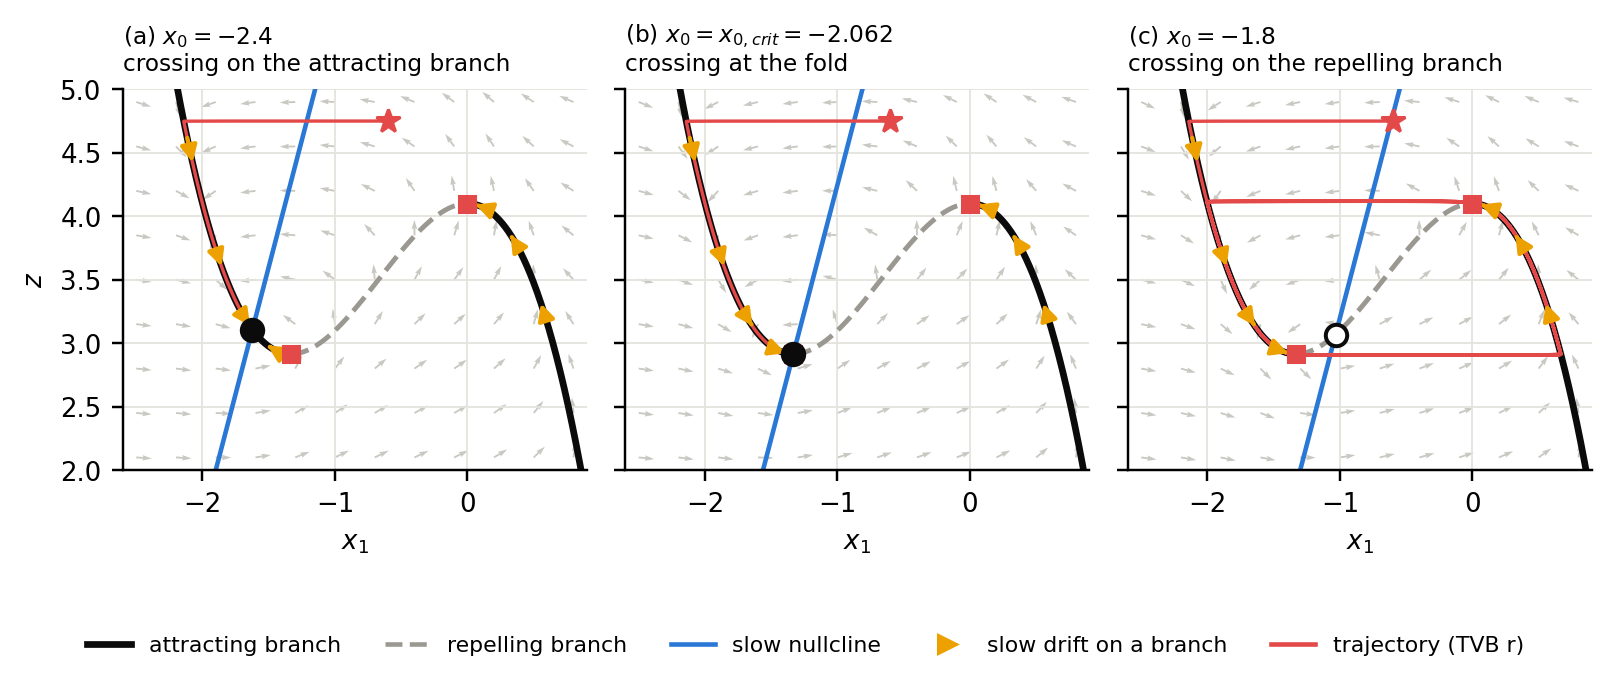
\includegraphics[width=\linewidth]{figs/pp_arrows.png}
\caption{The three cases of Fig.~\ref{fig:phase}, with the branches coloured by stability (solid: attracting; dashed:
repelling; red squares: folds), the slow drift along each attracting branch (orange), and one trajectory simulated with
TVB's $r$ from the star. (a) The drift on the interictal branch converges on the crossing: stable rest. (b) The crossing
sits on the fold: the critical case. (c) The whole interictal branch lies above the line, so the drift always points
down to the fold; there the branch ends, the state jumps to the ictal branch, climbs it to the top fold, jumps back:
a relaxation cycle (seizures). The fixed point (open circle) lies on the repelling branch.}\label{fig:pp}
\end{figure}

\subsubsection*{Step 4: why panel (c) has no stable rest state}
The arrows far from the curves are the same in (a) and (c): fast horizontal jumps onto the nearest attracting branch, which
do not depend on $x_0$. The difference is entirely in Step 3, in the sign of the gap on the interictal branch.
\begin{itemize}
\item \textbf{(a) $x_0 = -2.4$.} The line crosses the interictal branch at $x_1^* = -1.623$, $z^* = 3.107$. Above that point
the cubic is above the line ($\dot z<0$, slide down); between the crossing and the fold the cubic is below the line
($\dot z>0$, slide up). The drift converges on the crossing from both sides. The trajectory in Fig.~\ref{fig:pp}a lands on
the branch and stops there.
\item \textbf{(c) $x_0 = -1.8$.} The line has moved right; at the fold it is at $4(-4/3 + 1.8) = 1.87$, below the cubic's
$\zsn = 2.915$. Since the line is steeper than the branch, the cubic is above the line along the \emph{whole} interictal
branch: $\dot z<0$ everywhere on it (Fig.~\ref{fig:slow}a, orange curve: no zero crossing). The state slides down to the
fold, where the branch ends; the fast motion then carries it horizontally to the ictal branch (onset). There $x_1\approx 0.67$
and $4(x_1-x_0)\approx 9.9\gg z$, so $\dot z>0$: it climbs to the top fold at $z=4.1$, falls back to the interictal branch
(offset), and the loop repeats with a period of about 1760 model units, spending 47\% of the time on the interictal
branch (Fig.~\ref{fig:slow}b).
\end{itemize}
\textbf{The fixed point still exists in (c)}: the line crosses the cubic once for every $x_0$ (the line's slope, 4, is
steeper than the cubic's maximum slope, $G'(-2/3) = 4/3$). But it now lies on the repelling middle branch, at
$x_1^* = -1.033$, $z^* = 3.068$. There $G'(x_1^*) = +0.93$, and the Jacobian
\[
J = \begin{pmatrix} G'(x_1^*) & -1\\ 4r & -r \end{pmatrix}
\]
has eigenvalues $+0.929$ and $+0.0012$: an unstable node. A state placed exactly on it stays, but any offset in $x_1$ grows
as $e^{0.93\,t}$ and is pushed horizontally off the middle branch within a few time units. ``No rest state'' therefore
means: no \emph{stable} rest state.

\begin{figure}[H]\centering
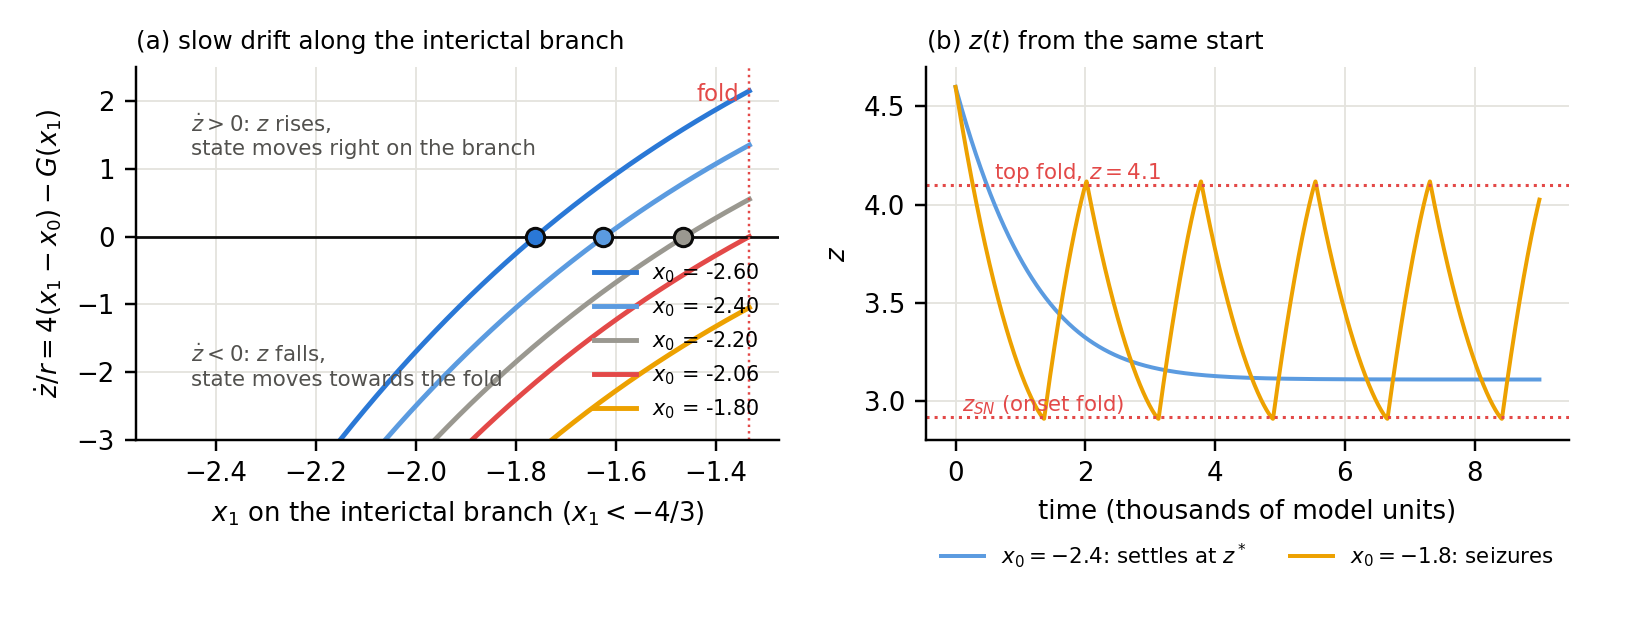
\includegraphics[width=\linewidth]{figs/pp_slowflow.png}
\caption{(a) The slow drift on the interictal branch, $\dot z/r = 4(x_1-x_0) - G(x_1)$, against the position on the branch.
A zero (dot) is a fixed point; positive values push $z$ up, negative ones down towards the fold (dotted). As $x_0$ increases
the curve moves down, the zero moves right, reaches the fold at $\xc$ (red) and disappears ($x_0=-1.8$, orange: negative
everywhere). (b) $z(t)$ from the same start: relaxation to $z^*$ for $x_0=-2.4$; sawtooth between $\zsn$ and 4.1 for
$x_0=-1.8$.}\label{fig:slow}
\end{figure}

\subsubsection*{Step 5: what moves the fixed point onto the repelling branch}
Nothing in the fast dynamics changes with $x_0$; only the slow nullcline moves. The fixed point solves
$G(x_1) = 4(x_1 - x_0)$, i.e.
\[
x_0 = x_1^* - \frac{G(x_1^*)}{4}.
\]
\textbf{It moves steadily to the right.} Differentiating,
\[
\frac{dx_0}{dx_1^*} = 1 - \frac{G'(x_1^*)}{4}\quad\Rightarrow\quad \frac{dx_1^*}{dx_0} = \frac{4}{4 - G'(x_1^*)} > 0,
\]
positive everywhere because $G'\le4/3<4$. As $x_0$ increases, the line slides right and its crossing with the cubic slides
continuously along the cubic: down the interictal branch, through the fold, and up the repelling middle branch
(Fig.~\ref{fig:fpmove}a,b). Near the fold, $dx_1^*/dx_0 \to 1$: the fixed point moves at the same speed as $x_0$. The fold is
reached exactly when $x_0 = x_1^* - G(x_1^*)/4$ with $x_1^* = -4/3$, which is $\xc = -2.062$ (Eq.~\ref{eq:xc}).

\textbf{Its stability follows its position.} Along the path, $\det J = r(3x_1^{*2} + 4x_1^* + 4) > 0$ always, and
$\operatorname{tr} J = G'(x_1^*) - r$. So the sign of $G'$ at the fixed point, i.e.\ \emph{which branch it sits on}, decides stability:
\begin{itemize}
\item On the interictal branch ($G'<0$): $\operatorname{tr} J<0$, stable. The two eigenvalues are real and very different
(Fig.~\ref{fig:fpmove}c): a fast one, $\lambda_f\approx G'(x_1^*)$ (return onto the branch), and a slow one,
$\lambda_s\approx\det J/\lambda_f = -r\,(1 + 4/|G'|)$ (sliding along the branch). For $x_0 = -2.4$: $-1.41$ and $-0.0013$.
The fixed point is a \emph{stable node} with one fast and one slow direction.
\item Exactly at the fold ($G' = 0$): $\operatorname{tr} J = -r$, still very slightly stable; the two eigenvalues have merged into a
complex pair $-r/2 \pm i\sqrt{4r}\approx -0.0002\pm0.037i$: a weak focus.
\item Just past the fold, $\operatorname{tr} J$ changes sign when $G'(x_1^*) = r$, i.e.\ at $x_1^* = -4/3 + r/4$, which gives
$x_{0,H} = -2.06195$, only $9\times10^{-5}$ above $\xc$: a \textbf{Hopf bifurcation} (Fig.~\ref{fig:fpmove}d). For
$|x_0 - \xc|\lesssim0.019$ the eigenvalues are complex (the fixed point is a focus); outside that window they are real
again, and on the middle branch both are positive: an unstable node, as in panel (c).
\end{itemize}
Because $r$ is tiny, the Hopf and the fold coincide for practical purposes, and the cycle born at the Hopf grows almost
immediately into the full relaxation cycle of Step 4 (a canard explosion). So: \textbf{the fixed point becomes repelling
because increasing $x_0$ slides it through the fold onto the middle branch, where $G'>0$}.

\begin{figure}[H]\centering
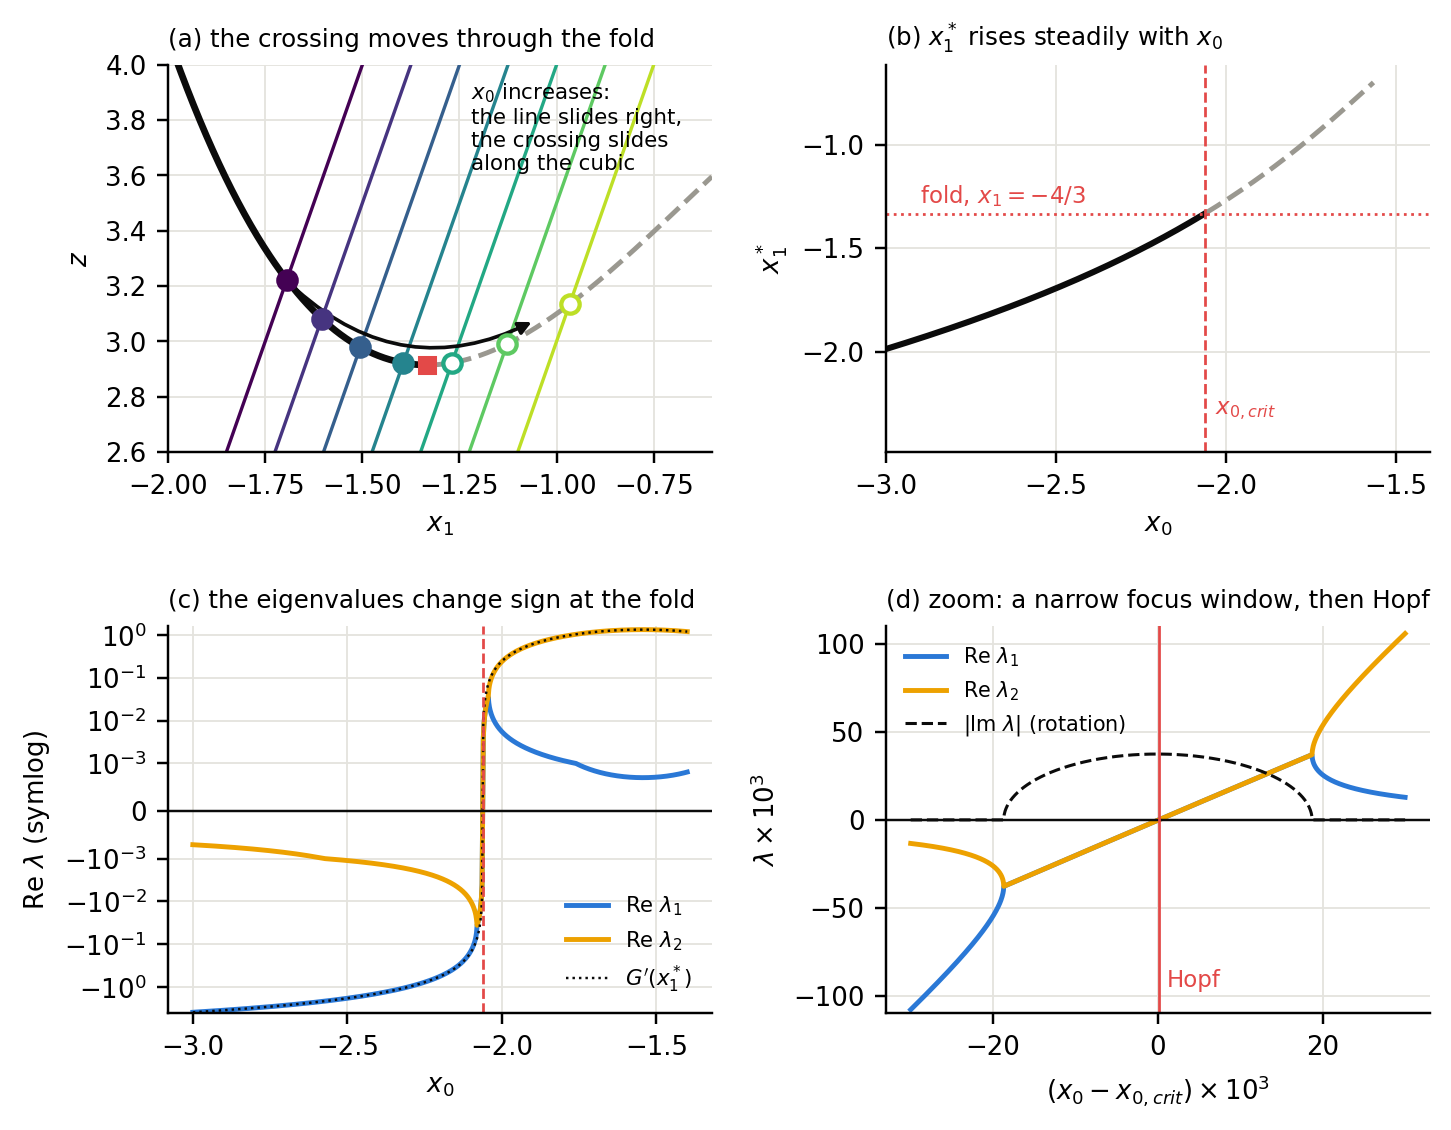
\includegraphics[width=\linewidth]{figs/pp_fpmove.png}
\caption{The fixed point as $x_0$ increases. (a) Slow nullclines for $x_0$ from $-2.5$ (dark) to $-1.75$ (yellow): the
crossing moves along the cubic, through the fold (red square), onto the repelling branch (open circles). (b) $x_1^*$ against
$x_0$ (this is Fig.~\ref{fig:bif}a): it rises monotonically and crosses the fold value $-4/3$ at $\xc$. (c) Real parts of
the two eigenvalues (symlog axis): one follows $G'(x_1^*)$ (dotted) and changes sign at the fold; the other is of order
$r$. (d) Zoom on $\pm0.03$ around $\xc$: in a window of width $\approx0.04$ the eigenvalues are complex (dashed: rotation
rate); their real part crosses zero at the Hopf point, $9\times10^{-5}$ above $\xc$.}\label{fig:fpmove}
\end{figure}

\subsubsection*{Reading Fig.~\ref{fig:bif} with this in mind}
Fig.~\ref{fig:bif} is the bifurcation diagram of the fixed point: one point $(x_1^*, z^*)$ for each $x_0$.
\begin{itemize}
\item \textbf{Panel (a), $x_1^*(x_0)$}, is the curve of Fig.~\ref{fig:fpmove}b: increasing, black (stable) while the fixed
point is on the interictal branch, grey (unstable) after it has passed the fold at $\xc$. There is a single branch and no
fold in this curve, because the 2D system never has more than one fixed point: the rest state does not \emph{collide} with
another fixed point and disappear, it \emph{changes stability} as it passes the fold of the fast nullcline.
\item \textbf{Panel (b), $z^*(x_0)$}, has a minimum at $\xc$. $z^* = G(x_1^*)$, and as $x_1^*$ moves right along the cubic,
$z^*$ follows the cubic down the interictal branch to its lowest point, the fold ($\zsn$), then up the middle branch. Near
the minimum, $z^* - \zsn\approx 2D^2$ with $D = \xc - x_0$ (Section~\ref{sec:nearfold}): $z^*$ hardly moves while $x_0$
approaches the threshold, which is why $z$ is a poor indicator of how close a region is to seizing.
\item \textbf{The dashed line at $\xc$} is the onset threshold: for $x_0<\xc$ the region rests at $(x_1^*, z^*)$; for
$x_0>\xc$ the fixed point is still drawn (grey), but the system does not stay on it; it runs the relaxation cycle of
Fig.~\ref{fig:pp}c around it.
\end{itemize}

\subsection{Relaxation oscillations: what a ``seizure'' is in the 2D model}
For $x_0 > \xc$ the trajectory follows a relaxation cycle (Fig.~\ref{fig:relax}a):
\begin{enumerate}
\item On the interictal branch, $4(x_1 - x_0) < z$, so $z$ decreases slowly while $x_1$ tracks the branch.
\item At $z=\zsn$ the branch ends: $x_1$ jumps (fast) to the ictal branch, $x_1\approx0.67$. \emph{Onset.}
\item On the ictal branch, $4(x_1 - x_0) \gg z$, so $z$ rises.
\item At $z = 4.1$ the ictal branch ends: $x_1$ jumps back to the interictal branch, $x_1 = -2$. \emph{Offset.}
\end{enumerate}
Fig.~\ref{fig:2d} shows the corresponding time series. Two properties matter for us.
\emph{Slow passage}: when $x_0$ is ramped slowly through $\xc$, onset occurs slightly after the crossing (the
trajectory stays near the vanishing rest state for a while), and seizures stop slightly after $x_0$ comes back
below $\xc$. \emph{Determinism}: without noise, the 2D Epileptor seizes as soon as, and as long as, $x_0 > \xc$.

\begin{figure}[H]\centering
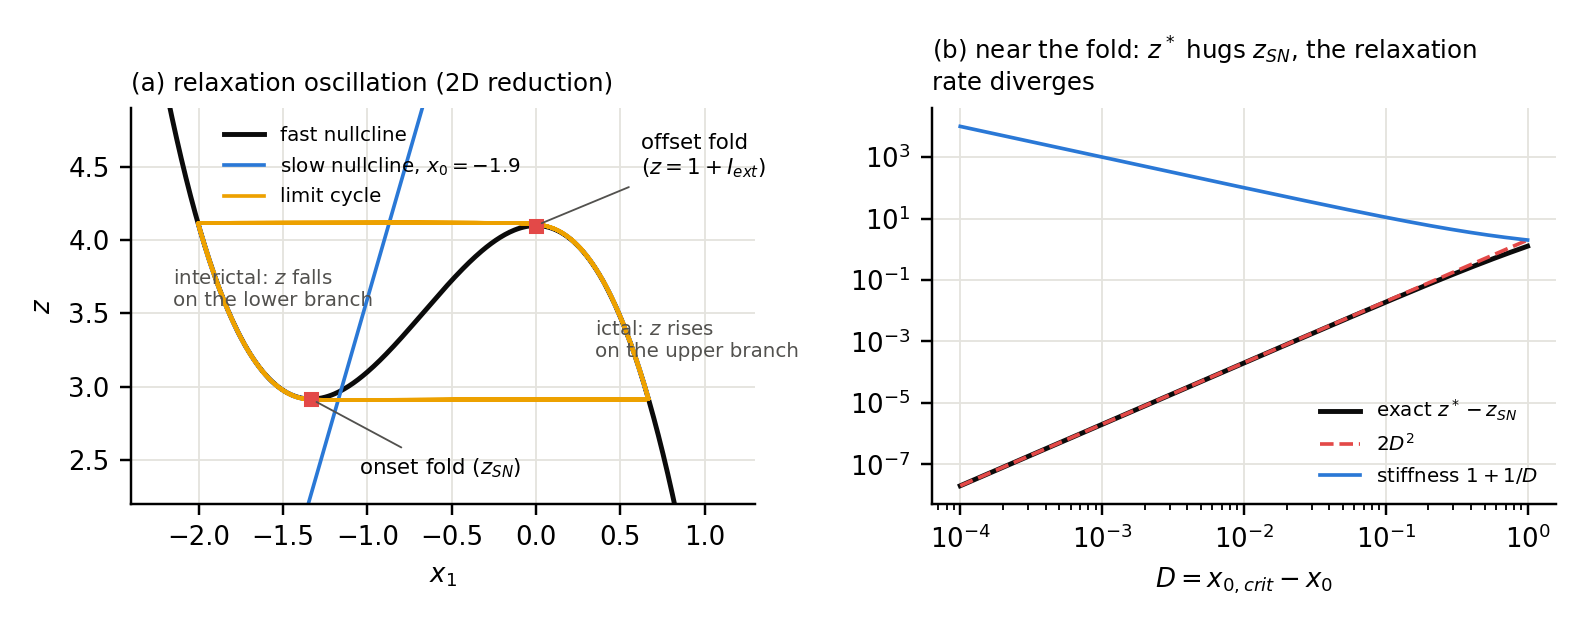
\includegraphics[width=\linewidth]{figs/th_relaxation.png}
\caption{(a) The 2D seizure cycle for $x_0=-1.9$. (b) Near the fold, the interictal fixed point lies only $2D^2$
above $\zsn$ (with $D = \xc - x_0$; Section~\ref{sec:nearfold}), and the effective relaxation rate of $z$ grows as
$1 + 1/D$: the dynamics become stiff precisely where the mapping is most interesting.}\label{fig:relax}
\end{figure}

\begin{figure}[H]\centering
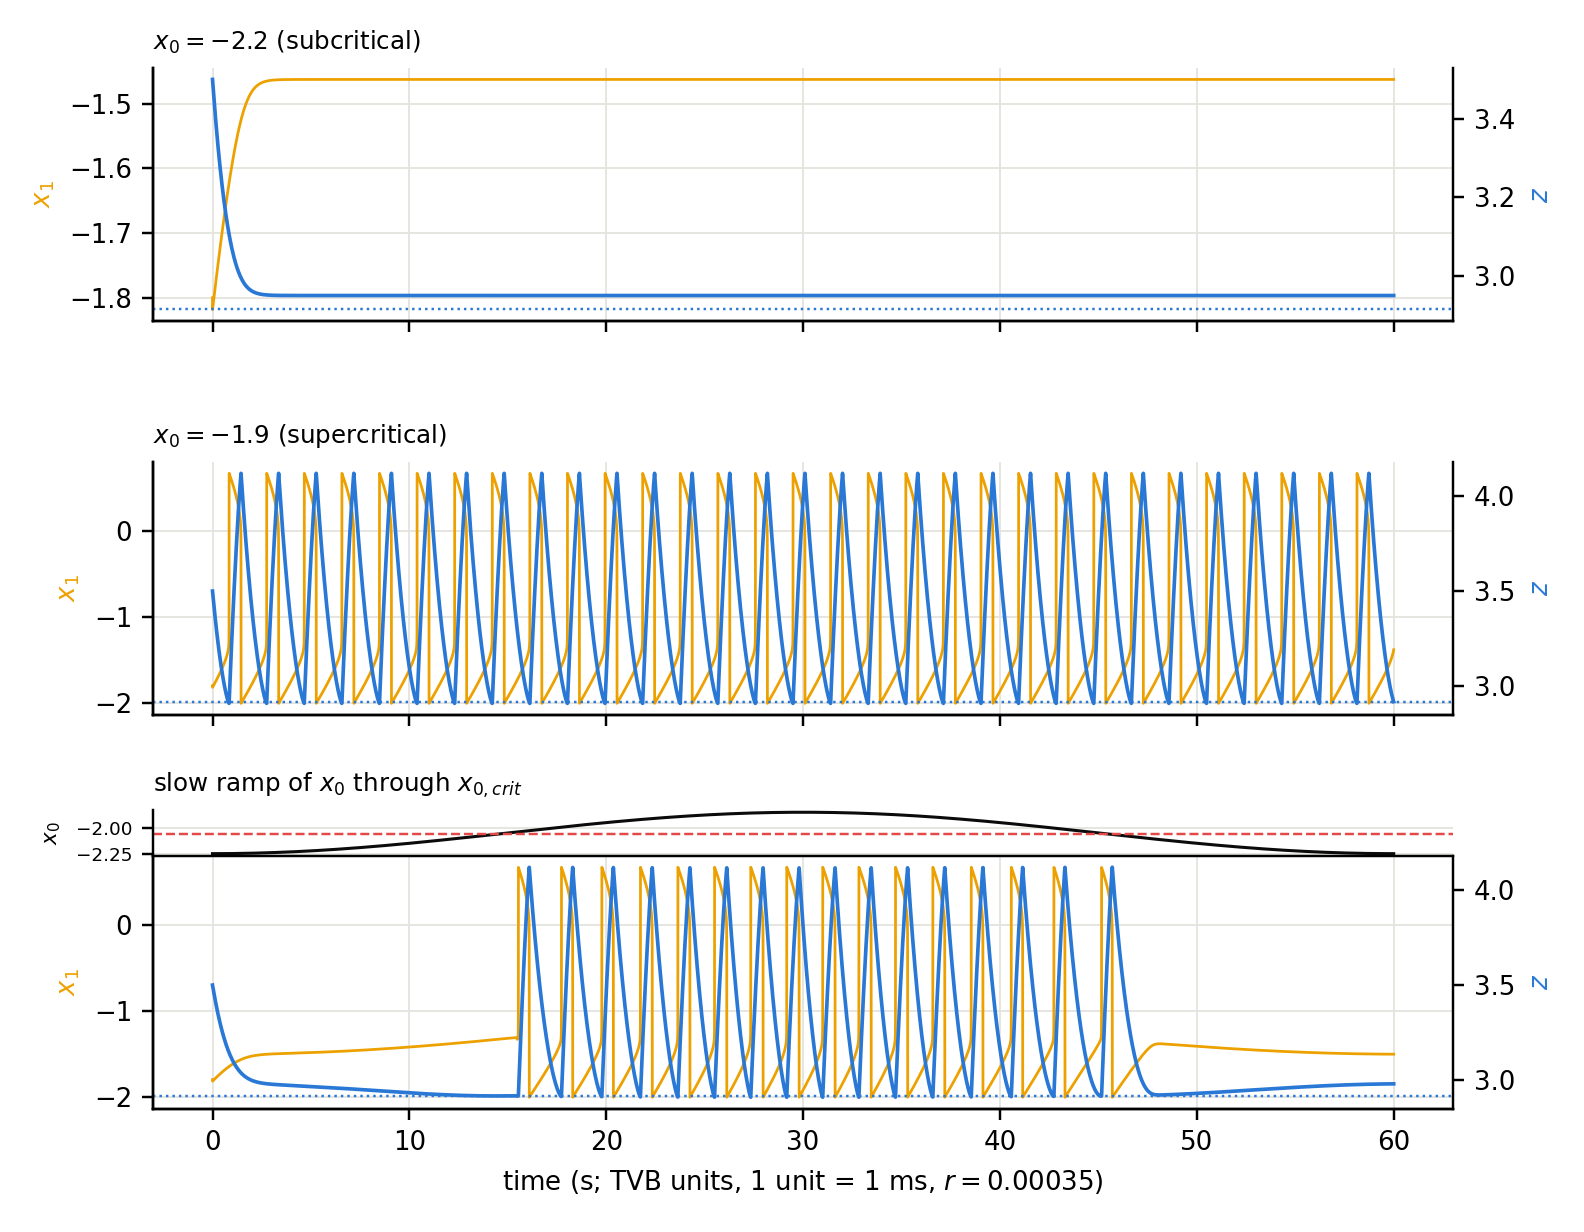
\includegraphics[width=0.95\linewidth]{figs/th_2d_sims.png}
\caption{2D Epileptor time series (TVB units). Top: subcritical, rest. Middle: supercritical, periodic seizures; $z$
oscillates between $\zsn$ (dotted) and 4.1. Bottom: $x_0$ ramped slowly through $\xc$ (inset): seizures start shortly
after the crossing and stop shortly after the return.}\label{fig:2d}
\end{figure}

\subsection{Behaviour near the fold}\label{sec:nearfold}
Near the fold, expand the fast nullcline: $G(x_1) \approx \zsn + 2u^2$ with $u = x_1 - \xsn$ (since $G''/2 = 2$).
With $D = \xc - x_0$ and \eqref{eq:xc}, the slow nullcline is $z = 4u + \zsn + 4D$. The interictal intersection solves
$2u^2 = 4u + 4D$, i.e.\ $u = 1 - \sqrt{1+2D} \approx -D$, so
\begin{equation}
z^* - \zsn \approx 2D^2,\qquad \frac{\partial x_1}{\partial z}\Big|_{\text{branch}} = \frac{1}{G'(x_1^*)} \approx -\frac{1}{4D}.
\end{equation}
With $x_1$ slaved to the branch, $\dot z = r[4(x_1(z) - x_0) - z]$ relaxes at rate $r(1 - 4\,\partial x_1/\partial z)
\approx r(1 + 1/D)$. Two consequences: (i) the interictal $z$ barely moves (by $2D^2$) while $x_0$ approaches the threshold,
so $z$ is a poor indicator of proximity to onset; (ii) numerically, explicit time steps overshoot across the fold when
$D$ is small, which we hit in practice (Section~\ref{sec:zint}).

\subsection{Time scales}\label{sec:timescales}
With TVB's $r$, $1/r\approx2.9$\,s. A 2D seizure (one passage up the ictal branch) lasts well under a second, and the
whole cycle a couple of seconds (Fig.~\ref{fig:2d}). In the full model, seizures last $\sim0.7$\,s in TVB units
(Fig.~\ref{fig:6d}). Fitted to patients, the time axis is stretched so that seizures last tens of seconds.
Our network's seizures last about a minute, and its HSP changes over thousands of seconds.

%==========================================================================================
\section{The HSP network seen as a slow--fast system}
%==========================================================================================
\subsection{Reminder of the model}
100 conductance-based LIF excitatory cells and 25 inhibitory cells; each E cell receives its own Poisson drive
(36\,Hz deafferented, 40\,Hz healthy). HSP acts on each E cell's recurrent AMPA and GABA conductances through
gains $\kA,\kG\in[0,1]$:
\begin{equation}
\dot \kA = \frac{(1-\kA)\,G_\uparrow(\hat r)}{\tau^{A}_{ins}} - \frac{\kA\,G_\downarrow(\hat r)}{\tau^{A}_{int}},\qquad
\dot \kG = \frac{(1-\kG)\,G_\downarrow(\hat r)}{\tau^{G}_{ins}} - \frac{\kG\,G_\uparrow(\hat r)}{\tau^{G}_{int}}.
\label{eq:hsp}\end{equation}
$\hat r$ is the cell's rate estimate, a leaky spike count: $\tau_{HSP}\,\dot{\hat r} = -\hat r + \sum_k\delta(t-t_k)$, with
$\tau_{HSP} = 100$\,s. The gates are smooth sigmoids around a target $r_0 = 2$\,Hz,
$G_\uparrow = \sigma\big(15[(r_0-\hat r)/r_0 - \tfrac12]\big)$ (half-on at 1\,Hz) and
$G_\downarrow = \sigma\big(15[(\hat r-r_0)/r_0 - \tfrac12]\big)$ (half-on at 3\,Hz). They are never exactly zero: near
2\,Hz both are about $10^{-3}$, so the gains always drift slowly. The analysis below uses runs with all four time
constants equal to 250\,s.

\subsection{Its cycle in slow--fast language}\label{sec:slowfast}
\begin{itemize}
\item \textbf{Fast subsystem}: the spiking network at fixed $(\kA, \kG)$. For moderate gains it has a low-rate state
($\sim1$\,Hz). Near $\kA\to1$, $\kG\to0$ it becomes \emph{bistable}: a saturated state (hundreds of Hz) coexists with the
low-rate one, and input noise can kick the network from one to the other. With HSP frozen at the state 5\,min before
an onset, half of the probe runs ignited.
\item \textbf{Slow subsystem}: $(\kA,\kG)$. Under the 36\,Hz drive the network fires about 1.2\,Hz, below target, where
$G_\uparrow\approx0.2$. HSP keeps inserting AMPA and removing GABA, carrying the fast subsystem towards its bistable
region.
\item \textbf{Onset} of the high-rate state: a noise-triggered jump once the low-rate state has become fragile.
\item \textbf{End}: in the high-rate state $\hat r$ rises far above 3\,Hz, $G_\downarrow$ saturates and HSP removes AMPA
at its maximal rate. The high-rate state disappears; $\hat r$ stays high for several minutes after the firing has
dropped (the rate filter lags), so AMPA keeps being removed, and the network ends in a deep, long quiet state from which
HSP recovers over about an hour.
\end{itemize}
In compressed time, each high-rate state lasts about a minute and looks like a single long seizure. With realistic
time constants it becomes a high-risk period of days. The question for the Epileptor is therefore not which of its
variables reproduces the high-rate state, but which one carries the slow change of risk. That is $x_0$
(Section~\ref{sec:why}).

\begin{table}[H]\centering\small
\begin{tabular}{p{3.6cm}p{5.4cm}p{5.6cm}}
\toprule
 & Epileptor (2D) & HSP network \\
\midrule
fast state & $x_1$ & population firing state (low-rate / high-rate) \\
excitability & parameter $x_0$ (fixed per region) & set by $\kA$, slowly varying \\
slow clock of each seizure & $z$ (rate $r$) & not represented: the network has no seizure-scale variable \\
high- / low-risk periods & not represented ($x_0$ fixed) & the HSP cycle \\
\bottomrule
\end{tabular}
\caption{What each model provides. The mapping gives the Epileptor the slow, HSP-driven change of $x_0$ that it does not
have, and gives the network the seizure-scale clock $z$ that it does not have.}
\end{table}

%==========================================================================================
\section{The mapping, step by step}
%==========================================================================================
\begin{figure}[H]\centering
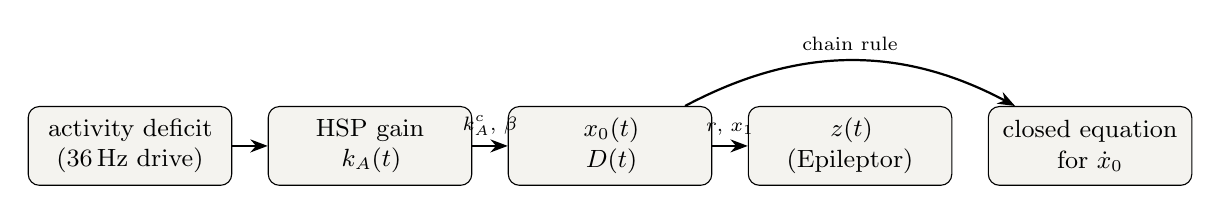
\begin{tikzpicture}[node distance=0.55cm and 0.45cm, every node/.style={font=\small},
  box/.style={draw, rounded corners, fill=boxc, align=center, minimum height=1.0cm, text width=2.35cm},
  arr/.style={-{Stealth[length=2.2mm]}, thick}]
\node[box] (d) {activity deficit\\(36\,Hz drive)};
\node[box, right=of d] (h) {HSP gain\\$\kA(t)$};
\node[box, right=of h] (x0) {$x_0(t)$\\$D(t)$};
\node[box, right=of x0] (z) {$z(t)$\\(Epileptor)};
\node[box, right=of z] (ode) {closed equation\\for $\dot x_0$};
\draw[arr] (d) -- (h); \draw[arr] (h) -- node[above, font=\scriptsize]{$\kA^c$, $\beta$} (x0);
\draw[arr] (x0) -- node[above, font=\scriptsize]{$r$, $x_1$} (z);
\draw[arr] (x0) to[bend left=28] node[above, font=\scriptsize]{chain rule} (ode);
\end{tikzpicture}
\caption{The chain of the mapping. GABA is left out because its weight, measured on the spiking network, is
negligible (Section~\ref{sec:Hderiv}).}
\end{figure}

\subsection{Why map HSP to $x_0$ rather than to $z$}\label{sec:why}
The 2D Epileptor has two slow quantities, and they do different jobs (Section~\ref{sec:fold}):
\begin{itemize}
\item $x_0$ is a \emph{parameter}. It sets where the slow nullcline $z=4(x_1-x_0)$ lies, and therefore whether the fixed
point sits on the interictal branch ($x_0<\xc$: the region rests) or not ($x_0>\xc$: the region seizes on its own).
\item $z$ is a \emph{state variable} with rate $r$. It runs each seizure: it falls slowly on the interictal branch, onset
happens when it reaches $\zsn$, it rises on the ictal branch, and offset happens when it reaches 4.1.
\end{itemize}
Three properties decide which one the HSP state corresponds to.

\textbf{(i) What HSP changes.} HSP multiplies the recurrent synaptic conductances. It therefore changes how strongly the
network amplifies its own activity, and so whether a low-rate state can turn into runaway activity without any change
of input. This is what $x_0$ encodes (rest exists or not), not what $z$ encodes (where the system is inside a seizure).

\textbf{(ii) How HSP moves in time.} Between two high-rate states, $\kA$ rises over about an hour, monotonically and
without any fast component: the behaviour of a slowly varying parameter. $z$ cannot play that role, because on these
time scales it is not free: on the interictal branch it relaxes to its fixed point $z^*(x_0)$ at rate $r(1+1/D)\ge r =
0.35$\,s$^{-1}$ (Section~\ref{sec:nearfold}), within seconds, while HSP takes thousands of seconds. Between seizures,
$z(t)\approx z^*(x_0(t))$: $z$ follows whatever $x_0$ does and carries no information of its own.

\textbf{(iii) What remains testable.} If HSP sets $x_0(t)$, then $z(t)$ is not chosen but computed from the Epileptor
equation, and whether it behaves sensibly is a test, not an assumption.

\subsection{Why the excitatory gain alone, and why its logarithm}\label{sec:Hderiv}
We want one number that measures how far the HSP state pushes the network towards higher activity, and we want the
relative weight of AMPA and GABA to come from the spiking network itself, not from a choice. The construction has six
steps; steps 1--4 measure the weights, step 5 shows that GABA can be dropped, step 6 explains the logarithm.

\paragraph{Step 1: the function that is measured.}
Freeze HSP (all four time constants set to $10^{99}$\,s), set every E cell's gains to $(\kA,\kG)$, drive the network at
36\,Hz and measure its mean E rate $\bar r_E(\kA,\kG)$ over 200\,s after a 20\,s transient. Freezing is needed because
otherwise the gains move during the measurement. Runs in which the frozen network ignites (E rate $>10$\,Hz in a 1\,s
bin) never come back and say nothing about the local rate response; they are excluded and counted.

\paragraph{Step 2: first-order expansion around a reference state.}
With $(\kA^{ref},\kG^{ref})$ the median interictal state of seed 1 (0.926, 0.071),
\[
\bar r_E \approx \bar r_E^{ref} + S_A\,\Delta\kA + S_G\,\Delta\kG,\qquad
S_A = \frac{\partial\bar r_E}{\partial\kA},\quad S_G = \frac{\partial\bar r_E}{\partial\kG},
\]
with the expected signs $S_A>0$ and $S_G<0$.

\paragraph{Step 3: compare relative changes.}
$S_A$ and $S_G$ are in Hz per unit of gain, and the two gains have very different sizes: a step of 0.01 is 1.1\% of
$\kA$ but 14\% of $\kG$. The comparable quantity is the response to the same \emph{relative} change of each gain, i.e.\
to scaling all AMPA (or all GABA) synapses by the same factor, which is what synaptic scaling does. A relative change is
$\Delta k/k^{ref}$, so
\[
\Delta\bar r_E \approx S_A\,\Delta\kA = \underbrace{(\kA^{ref} S_A)}_{q_A}\,\frac{\Delta\kA}{\kA^{ref}},\qquad
\Delta\bar r_E \approx S_G\,\Delta\kG = -\underbrace{(-\kG^{ref} S_G)}_{q_G}\,\frac{\Delta\kG}{\kG^{ref}} .
\]
The same rate change is written twice: once per unit of gain (slope $S$), once per relative change (slope $q = k^{ref}S$).
The factor $1/k^{ref}$ goes into the change and the factor $k^{ref}$ into the slope; they cancel.

\paragraph{Step 4: measurement.}
Central differences in the relative perturbation $\delta$:
$q_A = [\bar r_E(\kA^{ref}(1+\delta)) - \bar r_E(\kA^{ref}(1-\delta))]/(2\delta) + O(\delta^2)$ (the second-order terms cancel
in the difference), and likewise for GABA. The $+$ and $-$ runs share their Poisson input (common random numbers), so
the input noise largely cancels in the difference. Results are in Table~\ref{tab:sens} and Fig.~\ref{fig:sensdelta}. At
$\delta = 2\%$: $S_A = 0.793$\,Hz, $q_A = 0.734$\,Hz; $S_G = -0.035$\,Hz, $q_G = 0.0025$\,Hz.

\begin{table}[H]\centering\footnotesize
\setlength{\tabcolsep}{3.5pt}
\begin{tabular}{lcccccccc}
\toprule
state & seed & $\delta$ & $\kA$ & $\kG$ & $\bar r_E$ (Hz) & $S_A$ (Hz) & $S_G$ (Hz) & $w_A$ \\
\midrule
median interictal & 1 & 1\% & 0.926 & 0.071 & 1.25 & $0.878\pm0.024$ & $-0.071$ & 0.994 \\
median interictal & 1 & 2\% & 0.926 & 0.071 & 1.25 & $0.793\pm0.016$ & $-0.035$ & \textbf{0.997} \\
median interictal & 1 & 5\% & 0.926 & 0.071 & 1.25 & $0.826\pm0.015$ & $+0.018\pm0.053$ & -- (sign) \\
median interictal & 1 & 10\% & 0.926 & 0.071 & 1.25 & ignites (2/10 runs) & $-0.016\pm0.027$ & -- \\
post-ictal (+300\,s) & 1 & 5\% & 0.229 & 0.771 & 0.94 & $0.255\pm0.001$ & $-0.0013$ & 0.983 \\
recovery (+1500\,s) & 1 & 5\% & 0.798 & 0.201 & 1.16 & $0.584\pm0.007$ & $-0.004$ & 0.998 \\
early build-up & 1 & 5\% & 0.928 & 0.063 & 1.25 & $0.846\pm0.012$ & $-0.136\pm0.056$ & 0.989 \\
pre-ictal ($-300$\,s) & 1 & 5\% & 0.972 & 0.025 & 1.29 & ignites (5/10 runs) & -- & -- \\
median, seeds 2--5 & 2--5 & 5\% & 0.89--0.93 & 0.07--0.11 & 1.22--1.25 & 0.73--0.80 & $-0.02$ to $-0.07$ & 0.993--0.997 \\
\bottomrule
\end{tabular}
\caption{Frozen-HSP rate sensitivities, with $w_A = q_A/(q_A+q_G)$. Error bars from two noise seeds (none shown when
both seeds gave the same spike counts).}\label{tab:sens}
\end{table}

\begin{figure}[H]\centering
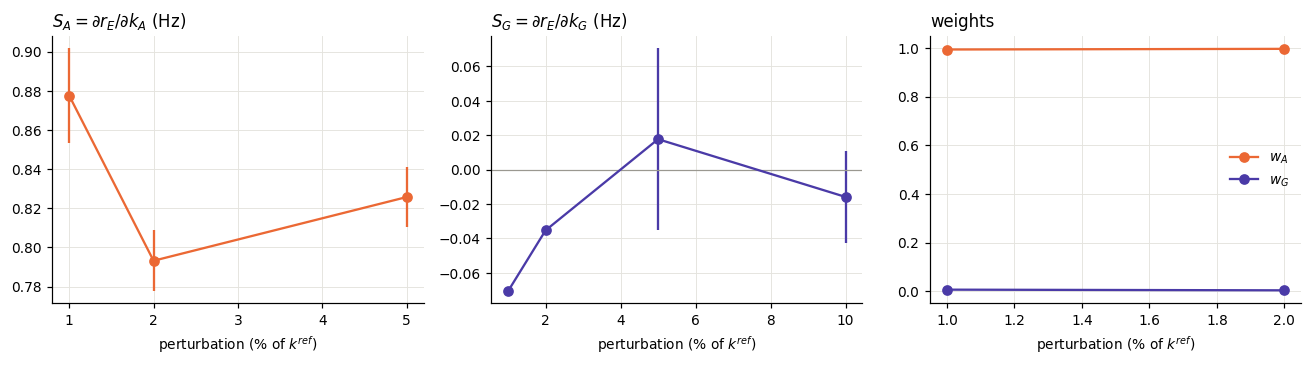
\includegraphics[width=0.95\linewidth]{figs/nb_cell12_0.png}
\caption{$S_A$, $S_G$ and the weights against perturbation size (seed 1, median interictal state). Points with an ignited
run are missing.}\label{fig:sensdelta}
\end{figure}

\paragraph{Step 5: GABA can be dropped.}
The normalised weights are $w_A = q_A/(q_A+q_G) = 0.997$ and $w_G = 0.003$. At every state and seed probed, $w_G$ is
between 0.002 and 0.017 (Table~\ref{tab:sens}). The reason is physical: on the plateau before a high-rate state, $\kG\approx
0.03$--$0.07$, so inhibition onto E cells is already almost gone and scaling it by a few percent barely changes the rate.
The GABA response is in fact at the resolution limit of the probe: at $\delta=2\%$ the rate difference $2\delta q_G =
10^{-4}$\,Hz is two spikes in the whole measurement (100 cells $\times$ 200\,s). What is robust is that it is small.
Keeping the GABA term would change $x_0$ by at most 0.008 anywhere on the cycle (Section~\ref{sec:res}); we therefore use
the excitatory gain alone. (Measuring the weights per unit of gain instead of per relative change gives $w_G = 0.043$:
still small, and again negligible on the untreated cycle.)

\paragraph{Step 6: where the logarithm comes from.}
Step 3 compares relative changes, $dk/k$. Summing small relative changes from a reference $k^{c}$ to $k$ gives the total
relative change:
\[
\int_{k^{c}}^{k}\frac{dk'}{k'} = \ln\frac{k}{k^{c}},\qquad\text{because}\qquad \frac{d\ln k}{dk} = \frac1k .
\]
For a small change this is the familiar relative change, $\ln(k/k^c) \approx (k-k^c)/k^c$; for large changes (over the
cycle $\kA$ goes from 0.16 to 0.98) the logarithm keeps adding up relative steps consistently, so that halving and
doubling count the same ($\pm\ln 2$). There is a second, dynamical reason. By the chain rule, $d\ln\kA/dt = \dot\kA/\kA$;
divide \eqref{eq:hsp} by $\kA$:
\[
\frac{d\ln\kA}{dt} = \frac{1-\kA}{\kA}\,\frac{G_\uparrow}{\tau^A_{ins}} - \frac{G_\downarrow}{\tau^A_{int}} .
\]
When the cell is over-active ($G_\uparrow\approx0$, $G_\downarrow\approx1$), $d\ln\kA/dt = -1/\tau^A_{int}$ exactly: AMPA
removal lowers $\ln\kA$ at a constant rate, whatever $\kA$. The logarithm is the coordinate in which removal is a uniform
drift (insertion is not: it is uniform in $\ln(1-\kA)$). Section~\ref{sec:ode} uses this.

\subsection{The threshold gain $\kA^c$}\label{sec:Hc}
The threshold is taken from the network's own onsets.
\begin{enumerate}
\item \textbf{Onsets.} $t_j$ is the first 1\,s bin of high-rate state $j$ with an E rate above 10\,Hz (12 onsets after the
500\,s settling, 5 seeds).
\item \textbf{Gain before each onset.} $\ln k_j = \mathrm{median}\{\ln\kA(t):\ t\in[t_j-300\,\mathrm s,\ t_j-2\,\mathrm s)\}$.
The window is long because $\kA$ barely moves on the late plateau; the last 2\,s are excluded because the gain already
reacts to the rising rate there. The 12 values of $e^{\ln k_j}$ range from 0.947 to 0.977.
\item \textbf{Threshold.} $\ln\kA^c = \mathrm{median}_j \ln k_j$, i.e.\ $\kA^c = 0.971$. It changes by less than 0.002
for windows of 100\,s (0.972) or 600\,s (0.970).
\item \textbf{Leave-one-out.} To ask whether $\kA$ approaches the threshold before onset $j$ without using onset $j$ to set
it, we use the median over the other 11 onsets.
\end{enumerate}

\subsection{The map: $x_0 = \xc + \beta\ln(\kA/\kA^c)$}\label{sec:map}
We need a map $\varphi$ from $\ln\kA$ to $x_0$ that is increasing (more excitable network, larger $x_0$) and sends the
network's threshold to the Epileptor's, $\varphi(\ln\kA^c) = \xc$. Expanding any smooth such map around the threshold
and keeping the first order gives the affine map, with $\beta = \varphi'>0$:
\begin{equation}\boxed{\;x_0(t) = \xc + \beta\,\ln\frac{\kA(t)}{\kA^c},\qquad D(t) = \xc - x_0(t) = \beta\,\ln\frac{\kA^c}{\kA(t)}\;}
\label{eq:map}\end{equation}
with $\xc = -2.062$ (Eq.~\ref{eq:xc}) and $\kA^c = 0.971$.

\textbf{What would fix $\beta$.} A second state with a justified Epileptor value would give
$\beta = (x_{0,2}-\xc)/\ln(k_2/\kA^c)$. The 40\,Hz network is the obvious candidate, but nothing assigns an Epileptor $x_0$
to ``healthy'': any value below $\xc$ is consistent with it never seizing. We set $\beta=1$ \emph{as a visual embedding}:
\begin{itemize}
\item the \textbf{sign} of $D$ (subcritical $>0$, supercritical $<0$) and the \textbf{ordering} of states do not depend on
$\beta$;
\item the \textbf{size} of $D$ in Epileptor units does, and so does everything that depends on it near the fold ($z^*-\zsn
\approx 2D^2$, relaxation rate $r(1+1/D)$);
\item $D$ is a distance to a bifurcation, \emph{not} a time to seizure.
\end{itemize}
\textbf{A built-in ceiling.} Since $\kA\le1$, $x_0\le\xc + \beta\ln(1/\kA^c) = -2.033$ for $\beta=1$. HSP can push a region
just past the threshold, which is enough for the Epileptor to seize, and no further.

\subsection{$x_0$ as a dynamical variable driven by HSP}\label{sec:ode}
Because \eqref{eq:map} is a fixed function of $\kA$, $x_0$ inherits the HSP dynamics. This is the form needed to put HSP
into an Epileptor network.

\textbf{Derivation.} Differentiate \eqref{eq:map} with the chain rule ($\xc$, $\beta$, $\kA^c$ are constants):
\[
\dot x_0 = \beta\,\frac{d}{dt}\ln\kA = \beta\,\frac{\dot\kA}{\kA} .
\]
Insert the HSP equation \eqref{eq:hsp} for $\dot\kA$ and divide by $\kA$:
\[
\dot x_0 = \beta\left[\frac{1-\kA}{\kA}\,\frac{G_\uparrow(\hat r)}{\tau^A_{ins}} - \frac{G_\downarrow(\hat r)}{\tau^A_{int}}\right].
\]
Finally eliminate $\kA$ by inverting \eqref{eq:map}, $\kA = \kA^c\,e^{(x_0-\xc)/\beta}$, so that
$(1-\kA)/\kA = e^{-(x_0-\xc)/\beta}/\kA^c - 1$:
\begin{equation}\boxed{\;\dot x_0 = \beta\left[\Big(\frac{e^{-(x_0-\xc)/\beta}}{\kA^c} - 1\Big)\frac{G_\uparrow(\hat r)}{\tau_{ins}}
- \frac{G_\downarrow(\hat r)}{\tau_{int}}\right],\qquad \tau_{HSP}\,\dot{\hat r} = -\hat r + \text{(firing of the region)}\;}
\label{eq:ode}\end{equation}
(dropping the superscript $A$). $x_0$ now obeys a closed equation driven only by the region's rate estimate; no gain has
to be stored. The HSP time constants appear directly in it.

\textbf{Three regimes.}
\begin{itemize}
\item \textbf{Over-active} ($G_\downarrow\approx1$, $G_\uparrow\approx0$): $\dot x_0 = -\beta/\tau_{int}$, a constant speed.
In the network, the high-rate state plus the minutes during which $\hat r$ is still above 3\,Hz last about $64+380 =
444$\,s, which predicts a drop of $444/250 = 1.78$, from $-2.06$ to $-3.84$. The observed minimum is $-3.85$.
\item \textbf{Quiet} ($G_\uparrow = g>0$, $G_\downarrow\approx0$): $\dot x_0 = \beta\,(g/\tau_{ins})\,(e^{-(x_0-\xc)/\beta}/\kA^c - 1)$.
This is fast when $x_0$ is far below the threshold (the exponential is large) and slows down near the ceiling, where it
vanishes. Linearising near the ceiling gives a time constant $\tau_{ins}/g$: with the network at 1.2\,Hz, $g\approx0.18$
and $\tau_{ins}/g\approx1400$\,s, the slow final approach to the threshold.
\item \textbf{Near target} (both gates $\sim10^{-3}$): $x_0$ settles where the two terms balance. This is the healthy
network's fixed $x_0\approx-2.32$.
\end{itemize}

\textbf{Three time scales in one region.}
\begin{center}\small
\begin{tabular}{lll}
\toprule
variable & role & time scale \\
\midrule
$x_1$ & seizure activity & fast (the Epileptor's unit time) \\
$z$ & starts and stops each seizure & $1/r$ \\
$\hat r$, $x_0$ & rate sensor; excitability set by HSP & $\tau_{HSP}$; $\tau_{ins}$, $\tau_{int}$ (days in vivo) \\
\bottomrule
\end{tabular}
\end{center}

\textbf{Two caveats.} (i) The network's mapping uses the E-mean gain, while \eqref{eq:hsp} holds per cell. Equation
\eqref{eq:ode} is exact for one cell and approximate for the mean, which is accurate here because the cells' gains move
almost together. (ii) In an Epileptor network, ``the firing of the region'' must be read from the Epileptor's own
variables (for example a rate assigned to the interictal and ictal branches of $x_1$). That conversion is a modelling
choice to be made when moving to TVB; the mapping itself does not depend on it.

\subsection{What plays the role of $x_1$}
The $z$ equation needs $x_1(t)$, but the network has no Epileptor variable. Instead of building one from the firing rate,
which would need an arbitrary midpoint and amplitude, $x_1$ is the Epileptor's own coordinate and the network's
detector only chooses the branch. For a given $z$, the fast nullcline condition $G(x_1)=z$ is the cubic
$-x_1^3 - 2x_1^2 + 1 + I_{ext} - z = 0$. For $\zsn < z < 4.1$ it has three real roots: a lower one ($x_1<-4/3$, interictal
branch, attracting), a middle one ($-4/3<x_1<0$, repelling) and an upper one ($x_1>0$, ictal branch, attracting).
\[
x_1(t) = \begin{cases} \text{lower root at } z(t), & \text{detector: low-rate state},\\
\text{upper root at } z(t), & \text{detector: high-rate state.}\end{cases}
\]
If the requested branch does not exist at the current $z$, $x_1$ is held at that branch's fold and the sample is flagged.

\subsection{Reconstructing $z(t)$}\label{sec:zint}
\[
\dot z = r\,h(z,t),\qquad h(z,t) = 4\big(x_1(z,t) - x_0(t)\big) - z - 0.1 z^7\mathbf 1_{z<0},\qquad r = 0.35\ \mathrm{s}^{-1},
\]
with TVB's $r=0.00035$\,ms$^{-1}$ in seconds, $x_0$ linearly interpolated between 1\,s samples, and $z(0)$ at the
interictal fixed point.

\textbf{Why an explicit step fails.} Differentiating $G(x_1(z)) = z$ gives $dx_1/dz = 1/G'(x_1)$, and $G'\to0$ at the fold,
so $dx_1/dz$ diverges as $z\to\zsn$. An explicit step uses the slope at the start of the step, overshoots to $z<\zsn$ where
the lower branch no longer exists, and $z$ chatters across the fold (13\% of samples in a first implementation). The
interictal relaxation rate $r(1+1/D)$ is $0.35\times60 = 21$\,s$^{-1}$ for $D = 0.017$, so a 0.1\,s step spans two
relaxation times.

\textbf{Why backward Euler with bisection works.} The update $z_{n+1} = z_n + \Delta t\,r\,h(z_{n+1})$ is the root of
$F(z) = z - z_n - \Delta t\,r\,h(z)$. $h$ is strictly decreasing in $z$: on either attracting branch $dx_1/dz = 1/G'(x_1)$ with
$G'(x_1) = -x_1(3x_1+4) < 0$ (for $x_1<-4/3$ and for $x_1>0$); at a clamp this term is 0; $-z$ has derivative $-1$; and
$-0.1z^7\mathbf 1_{z<0}$ has derivative $-0.7z^6\le0$. So $F'\ge1+\Delta t\,r>0$: $F$ has exactly one root, found by
bisection. For a linearised $h=-\lambda(z-z^*)$ the backward-Euler factor $1/(1+\Delta t\,r\lambda)$ lies in $(0,1)$ for any
step: the scheme cannot overshoot. With $\Delta t = 0.1$\,s the interictal $z$ agrees with $\Delta t = 0.02$\,s to $10^{-5}$.

%==========================================================================================
\section{Results}\label{sec:res}
%==========================================================================================
Data: the long runs with all HSP time constants at 250\,s (15\,000\,s, 5 seeds), deafferented (36\,Hz) and healthy
(40\,Hz). 12 high-rate states in the deafferented network (2, 2, 3, 2, 3 per seed), none in the healthy one. Script:
\path{single_gain.py}.

\textbf{Single vs two gains.} $x_0$ from \eqref{eq:map} differs from the two-gain version (weights $w_A$, $w_G$ of
Table~\ref{tab:sens}) by at most 0.008 at any time, against a cycle range of 1.8. All numbers below are with the single
gain.

\begin{figure}[H]\centering
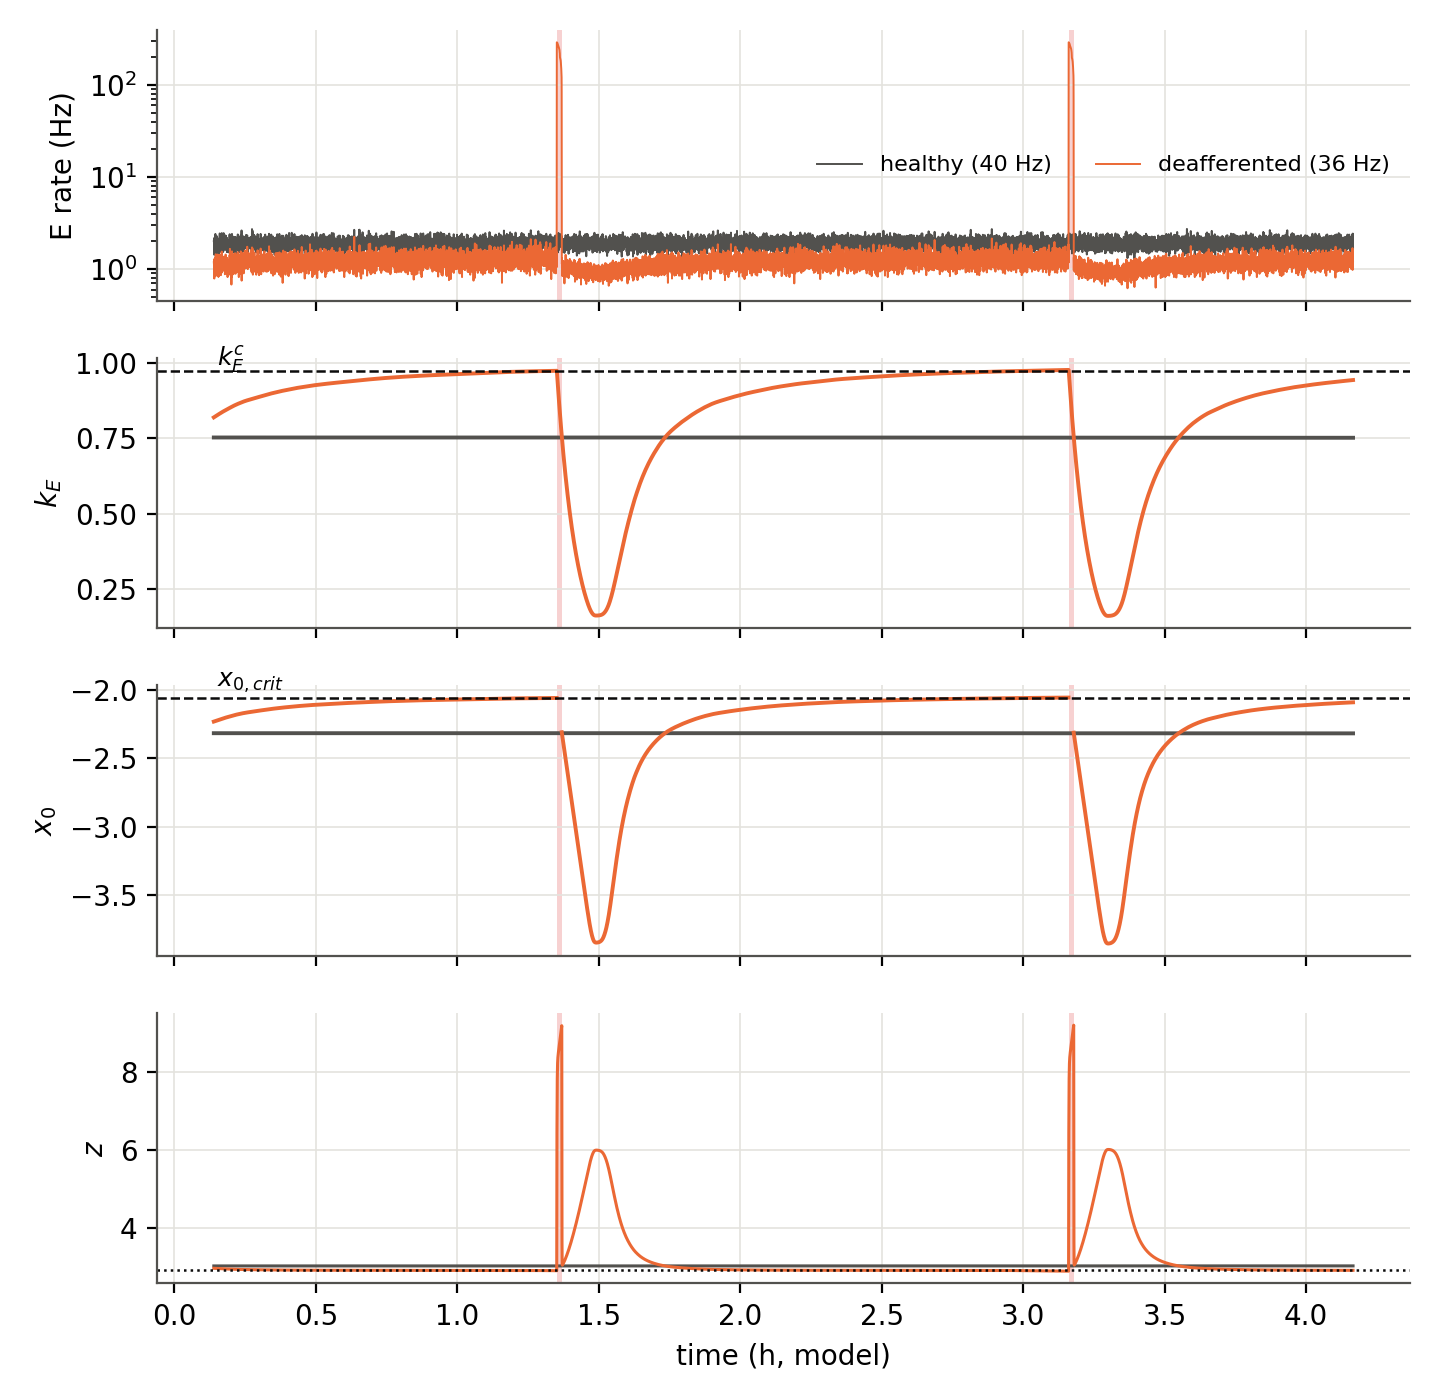
\includegraphics[width=0.85\linewidth]{figs/sg_timeseries.png}
\caption{Seed 1, deafferented (orange) vs healthy (grey). From top: E rate; excitatory gain $\kA$ with $\kA^c$; $x_0$
from \eqref{eq:map} (masked during high-rate states) with $\xc$; reconstructed $z$ with $\zsn$. Red bands: high-rate
states.}\label{fig:ts}
\end{figure}

\begin{figure}[H]\centering
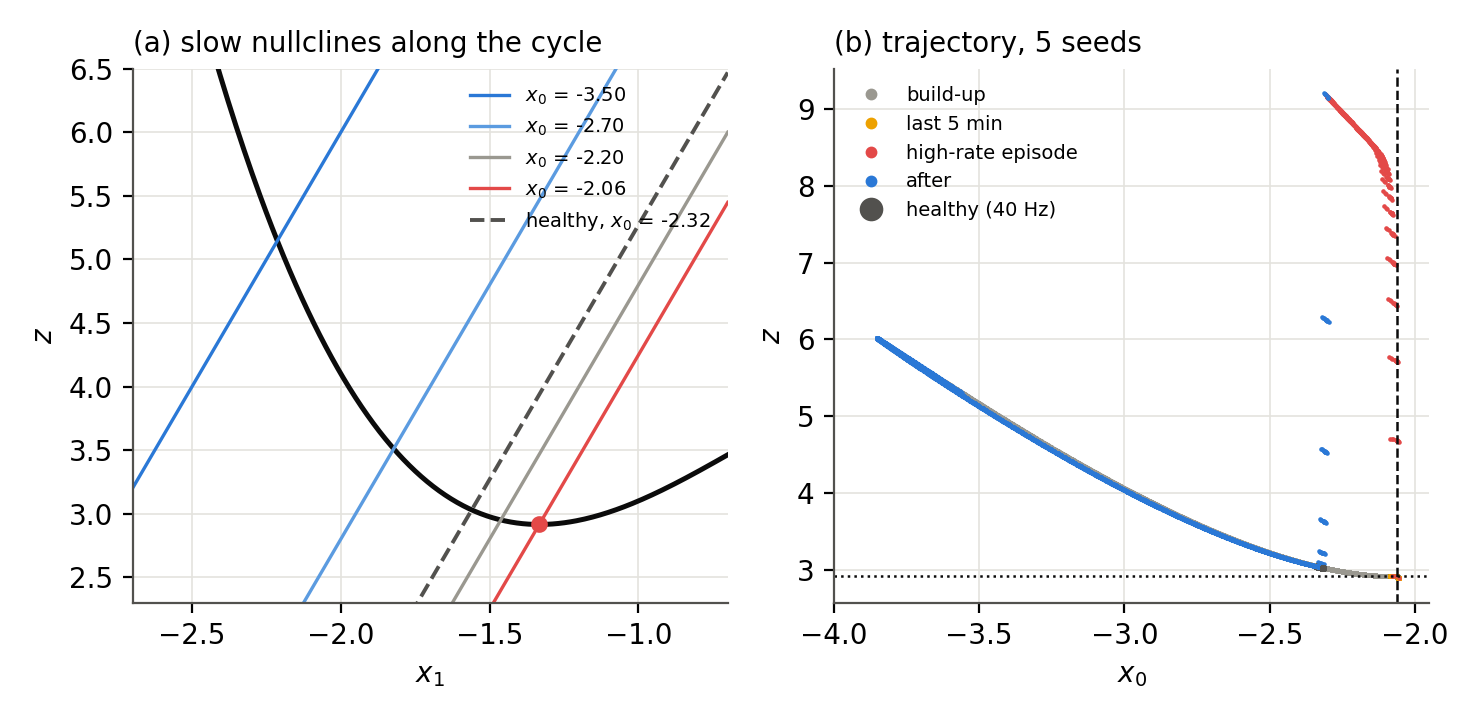
\includegraphics[width=\linewidth]{figs/sg_trajectory.png}
\caption{(a) Fast nullcline (black) and slow nullclines for values of $x_0$ visited along the deafferented cycle (blue:
just after a high-rate state; red: at the threshold) and for the healthy network (dashed); red dot: the fold.
(b) Trajectory of all 5 deafferented seeds in $(x_0, z)$, coloured by phase, and the healthy network. Dashed: $\xc$;
dotted: $\zsn$.}\label{fig:traj}
\end{figure}

\textbf{How to read Fig.~\ref{fig:traj}b.} The loop runs clockwise:
\begin{enumerate}
\item \emph{Build-up} (grey): $x_0$ rises slowly from about $-3.85$ to $\xc$ over about an hour, and $z$ follows its resting
value $z^*(x_0)$ down to $\zsn$.
\item \emph{Onset} (orange, then red) at $x_0\approx\xc$: the detector switches $x_1$ to the ictal branch and $z$ rises.
\item \emph{High-rate state} (red): during about a minute, HSP removes AMPA at its maximal rate, so $x_0$ falls to about
$-2.32$ while $z$ is high.
\item \emph{After} (blue): $z$ drops back onto the resting curve within seconds, and $x_0$ keeps falling for about 7\,min
(the rate sensor still reads a high rate) to $-3.85$; then the build-up starts again along the same curve.
\end{enumerate}
The healthy network sits at a single point on the same resting curve, $x_0 = -2.32$.

\subsection{The phase plane along the HSP cycle (poster panel 3B)}\label{sec:poster3b}
Panel 3B of the poster (and Fig.~\ref{fig:traj}a) applies Section~\ref{sec:pp} to the HSP cycle. The fast nullcline (black)
never changes; HSP only moves the slow nullcline, through $x_0(t)$. Fig.~\ref{fig:p3b} numbers the five moments shown
(seed 1).

\begin{figure}[H]\centering
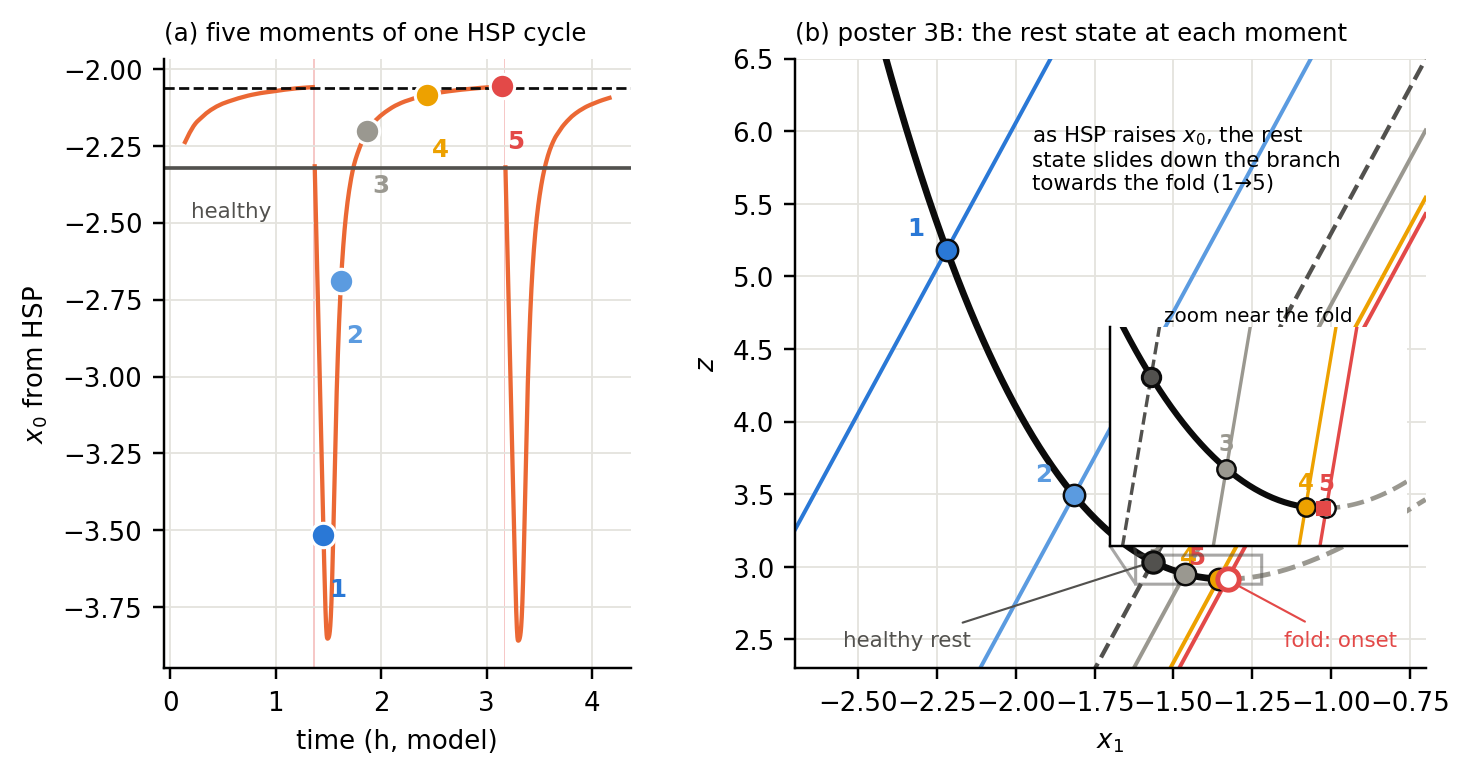
\includegraphics[width=\linewidth]{figs/pp_poster3b.png}
\caption{Poster panel 3B, explained. (a) $x_0(t)$ from the HSP state; red bands: high-rate states; numbered dots: the
moments drawn in (b). (b) For each moment, the slow nullcline (same colour) and its crossing with the cubic: the rest state
of the Epileptor at that moment. Dashed grey: the healthy network. Inset: the last three moments near the fold; moment 5 is
open because $x_0$ has just passed $\xc$.}\label{fig:p3b}
\end{figure}

\begin{center}\small
\begin{tabular}{clcccl}
\toprule
moment & time after the high-rate state & $x_0$ & rest state $(x_1^*, z^*)$ & slow eigenvalue & reading \\
\midrule
1 & 5\,min & $-3.515$ & $(-2.22,\ 5.18)$ & $-5.9\times10^{-4}$ & deep in the stable region \\
2 & 15\,min & $-2.689$ & $(-1.82,\ 3.49)$ & $-8.8\times10^{-4}$ & recovering \\
3 & 30\,min & $-2.201$ & $(-1.46,\ 2.95)$ & $-2.8\times10^{-3}$ & close to healthy \\
4 & 64\,min & $-2.085$ & $(-1.36,\ 2.916)$ & $-1.9\times10^{-2}$ & almost at the fold \\
5 & 107\,min (1\,min before onset) & $-2.057$ & $(-1.33,\ 2.915)$ & $+9.5\times10^{-3}$ & just past it: unstable \\
healthy & -- & $-2.324$ & $(-1.57,\ 3.03)$ & & fixed, stable \\
\bottomrule
\end{tabular}
\end{center}

\textbf{What happens, in Epileptor terms.}
\begin{enumerate}
\item \textbf{Right after a high-rate state} (moment 1), HSP has removed most of the excitation and $x_0$ is far below the
threshold. The line is far to the left and crosses the interictal branch high up ($z^*\approx5.2$). The region is deep in
the stable, low-risk regime: a perturbation would need to push $z$ down by more than 2 to reach the fold.
\item \textbf{During recovery} (moments 2--4), HSP raises $x_0$; the line slides right, and the rest state slides
\emph{down} the interictal branch towards the fold, quickly at first and then more and more slowly as HSP's insertion term
weakens near the ceiling. Because $z^*$ follows the cubic, which is flat near its minimum, the rest state almost stops
moving in $z$ ($z^* = 2.95$, then 2.916) even though $x_0$ still changes: the region is close to threshold but looks
almost the same.
\item \textbf{The slow eigenvalue grows}, from $-6\times10^{-4}$ to $-2\times10^{-2}$: the curve of Fig.~\ref{fig:fpmove}c
read from left to right. In the Epileptor, this is the approach to the fold seen from the fixed point (Step 5).
\item \textbf{One minute before onset} (moment 5), $x_0$ has just crossed $\xc$: the crossing has passed the fold onto
the repelling branch and the rest state is unstable. In the deterministic Epileptor, a seizure would start here. The spiking
network starts its high-rate state about a minute later: the onset is noise-triggered close to the fold, as discussed in
Section~\ref{sec:interp}.
\item \textbf{The healthy network} sits at one fixed line (dashed), whose crossing is on the interictal branch, between moments
2 and 3: subcritical, with $D = 0.26$. It never moves, because its HSP state does not drift.
\end{enumerate}
The whole HSP cycle is therefore a slow back-and-forth of the slow nullcline: far to the left after each high-rate state,
then slowly back to the fold. With realistic HSP time constants, the time spent near or past the fold (moments 4--5) is the
high-risk period.

\begin{table}[H]\centering\small
\begin{tabular}{lcccc}
\toprule
network & median $D$ & minimum $D$ & share $D<0$ & high-rate states \\
\midrule
deafferented (36\,Hz) & $+0.056$ & $-0.006$ & 4.5\% & 12 \\
healthy (40\,Hz) & $+0.256$ & $+0.252$ & 0 & 0 \\
\bottomrule
\end{tabular}
\caption{Distance to the Epileptor threshold on low-rate samples ($\beta=1$; signs meaningful).}\label{tab:D}
\end{table}

\begin{figure}[H]\centering
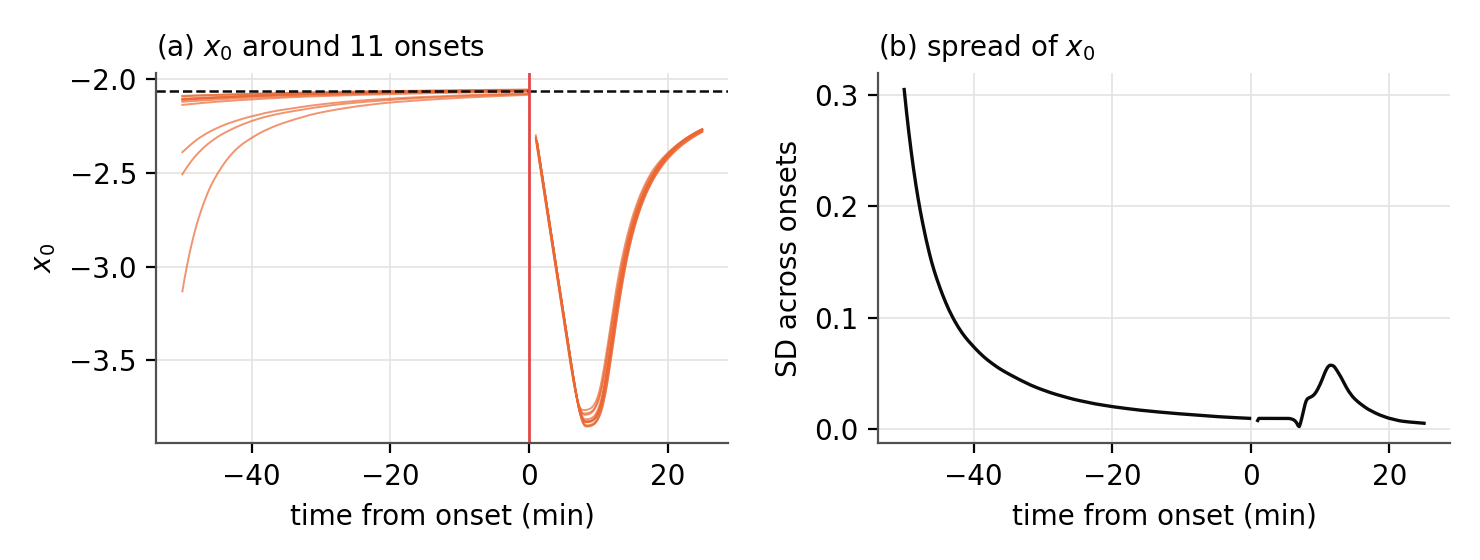
\includegraphics[width=\linewidth]{figs/sg_onsets.png}
\caption{(a) $x_0$ aligned on the onsets that have 50\,min of data before them (11 of 12). (b) Its SD across onsets.}
\label{fig:onsets}
\end{figure}

\textbf{Quantitative answers.}
\begin{enumerate}
\item \textbf{A repeatable loop.} Across onsets, $x_0$ differs by 0.017 (SD) at $-1000$\,s, 0.010 at $-100$\,s and 0.028 at
$+500$\,s, against a cycle range of 1.8 ($-3.85$ to $-2.06$).
\item \textbf{The healthy network stays subcritical}, in a narrow band at $D\approx+0.26$.
\item \textbf{$x_0$ reaches $\xc$ at onset.} With a leave-one-out threshold, the median $D$ at onset is $-0.001$. In 6 of 12
onsets, $D\le0$ was reached 8--19\,min before; the other 6 started while $D$ was still slightly positive (0.001--0.023).
\item \textbf{Closer before onsets.} In all 12, $D$ over the last 5\,min (median $0.000$) is smaller than 25--30\,min earlier
(median $+0.017$); Wilcoxon $p = 0.0005$.
\item \textbf{Moving away afterwards.} $D$ increases by a median of 1.35 over the first 10\,min after each high-rate state.
\item \textbf{$z$ is slaved to $x_0$ between high-rate states}: $|z - z^*(x_0)|$ is below 0.017 for 99\% of low-rate samples.
\item \textbf{Robustness.} $\kA^c$ changes by less than 0.002 for windows of 100--600\,s. Flagged samples ($x_1$ held at a
fold) make up 5.9\% of deafferented time: the 4.5\% of low-rate time at $D<0$ plus high-rate samples beyond the end of the
ictal branch.
\end{enumerate}

%==========================================================================================
\section{Interpretation}\label{sec:interp}
%==========================================================================================
\subsection{What the loop means}
Expressed as an Epileptor excitability, the HSP state carries the deafferented network back and forth through the
seizure threshold. After each high-rate state it throws $x_0$ deep into the subcritical region, and over about an hour it
brings it back to $\xc$. The path is the same in every cycle and every seed. In Epileptor terms, a deafferented region is
not a region with a fixed epileptogenic $x_0$: it is a region whose $x_0$ is a slow variable, regulated by homeostasis,
that \emph{returns to criticality}. The healthy region has a fixed $x_0$ below the threshold.

\subsection{The high-rate state as a high-risk period}
In compressed time, the network's high-rate state lasts about a minute, and the reconstructed $z$ does not fit it: $z$
climbs to about 9, far past the end of the ictal branch (4.1), where the Epileptor would already have ended a seizure.
This is a mismatch of time scales, not of mechanism. With realistic HSP constants (days), $x_0$ would stay above the
threshold for days during each high-risk period, and the Epileptor's own $z$, running at $1/r$, would generate a
\emph{cluster} of seizures during that time, each started and stopped by $z$. HSP would then do only the slow job: move
$x_0$ across the threshold and back. This division of labour (HSP for the risk, $z$ for each seizure) is what
Eq.~\eqref{eq:ode} provides, and what an Epileptor network with HSP would show.

\subsection{Deterministic threshold vs noisy onset}
The 2D Epileptor seizes as soon as $x_0>\xc$. The network spent up to 19\,min at $D<0$ before a high-rate state (4.5\% of
its low-rate time), and half of its onsets came slightly before $D$ reached zero. Both point to noise-triggered
transitions near a fold: with HSP frozen at the pre-onset state, half of the probe runs ignite. Near $\xc$ the network
has an onset \emph{rate}, not an onset time; in an Epileptor model, noise on $x_1$ or $z$ plays this role.

\subsection{What is anchored and what is not}
\begin{itemize}
\item \textbf{Anchored in the spiking model}: the irrelevance of GABA for the untreated cycle (local rate sensitivities),
the threshold gain $\kA^c$ (from the observed onsets, consistent with frozen-network ignition), the onset times.
\item \textbf{Anchored in the Epileptor}: $\xc$, $\zsn$ and the fold geometry, from its equations with TVB defaults.
\item \textbf{Phenomenological}: $\beta=1$ (the size of the $x_0$ axis), TVB's $r$ (which makes $z$ fast), and $x_1$ (the
canonical branch chosen by the detector, not a measured network variable).
\item \textbf{Left out}: inhibition. Dropping GABA is justified for the deafferented cycle, where $\kG$ stays small, but a
treatment that acts on inhibition (benzodiazepine-like) cannot be represented with this single-gain $x_0$.
\end{itemize}

%==========================================================================================
\section{Limitations and next steps}
%==========================================================================================
\textbf{Limitations.}
\begin{itemize}
\item One reference state for the sensitivities; the direction ($w_A\approx1$) is stable along the cycle, but the size of
the rate response is not, so $x_0$ orders states rather than predicting rates.
\item $\beta$ is uncalibrated, so distances in Epileptor units are not comparable with $x_0$ values inferred in patients.
\item $x_1$ is chosen by the detector; the mapping places observed onsets, it does not predict them.
\item Compressed time: HSP constants of minutes instead of days, so the high-rate state stands in for a whole high-risk
period.
\item Post hoc only: nothing is fed back into the network.
\end{itemize}

\textbf{Next steps}, towards TVB:
\begin{enumerate}
\item \textbf{One Epileptor with HSP.} Integrate the 2D (or full) Epileptor together with Eq.~\eqref{eq:ode} and the rate
sensor, with a rate read from $x_1$ and noise. Test whether high-risk periods with clusters of seizures appear when the
input to the region is lowered, and how their spacing scales with $\tau_{ins}$, $\tau_{int}$, $\tau_{HSP}$.
\item \textbf{Choose the rate readout.} Fix how a region's Epileptor activity is converted into the rate that HSP senses,
so that a healthy region sits at the 2\,Hz target and a deafferented one below it.
\item \textbf{TVB network.} Add $\hat r$ and $x_0$ as two extra state variables per region. Deafferent selected regions
(lower their input or their incoming connectivity) and study recruitment and propagation through the connectome.
\item \textbf{A second anchor for $\beta$}, for example by matching the frozen network's ignition probability against the
Epileptor's noise-driven onset rate as a function of $x_0$.
\item \textbf{Inhibition, later.} Add GABA back (a two-gain $x_0$ or an ignition-based weight) when treatments acting on
inhibition are studied.
\end{enumerate}

\appendix
\section{Implementation details}
\begin{itemize}
\item Single-gain analysis and the figures of Section~\ref{sec:res}: \path{epileptor/report/single_gain.py}
(reads \path{epileptor/results/trajectories.npz}).
\item Sensitivity probes and the export: \path{epileptor/HSP_Epileptor_trajectory.ipynb}; probe runner
\path{epileptor/hsp_epileptor_probe.py}; probe results cached in \path{epileptor/results/probes.json}.
\item Data: \texttt{spiking\_network/results/lfp\_tau250\_15k/raw/}: E-mean $\kA$, $\kG$ and E rate every 1\,s.
\item Fast-nullcline roots: closed-form cubic. $z$: backward Euler, $\Delta t=0.1$\,s, exact bisection.
\item Theory figures: \texttt{HSP\_Epileptor\_report/theory\_figures.py} (LSODA; TVB parameter values).
\item Previous version of this report (two-gain coordinate $H$, treatments): \path{report_v1.pdf}.
\end{itemize}

\begin{thebibliography}{99}\small
\bibitem{jirsa2014} V.~K. Jirsa, W.~C. Stacey, P.~P. Quilichini, A.~I. Ivanov, C.~Bernard. On the nature of seizure
dynamics. \emph{Brain} 137:2210--2230, 2014.
\bibitem{proix2014} T.~Proix, F.~Bartolomei, P.~Chauvel, C.~Bernard, V.~K. Jirsa. Permittivity coupling across brain
regions determines seizure recruitment in partial epilepsy. \emph{Journal of Neuroscience} 34:15009--15021, 2014.
\bibitem{jirsa2017} V.~K. Jirsa, T.~Proix, D.~Perdikis, et al. The Virtual Epileptic Patient: individualized whole-brain
models of epilepsy spread. \emph{NeuroImage} 145:377--388, 2017.
\bibitem{proix2017} T.~Proix, F.~Bartolomei, M.~Guye, V.~K. Jirsa. Individual brain structure and modelling predict
seizure propagation. \emph{Brain} 140:641--654, 2017.
\bibitem{saggio2020} M.~L. Saggio, D.~Crisp, J.~M. Scott, et al. A taxonomy of seizure dynamotypes. \emph{eLife}
9:e55632, 2020.
\bibitem{izhikevich2000} E.~M. Izhikevich. Neural excitability, spiking and bursting. \emph{International Journal of
Bifurcation and Chaos} 10:1171--1266, 2000.
\bibitem{sanzleon2013} P.~Sanz Leon, S.~A. Knock, M.~M. Woodman, et al. The Virtual Brain: a simulator of primate brain
network dynamics. \emph{Frontiers in Neuroinformatics} 7:10, 2013.
\bibitem{krupa2001} M.~Krupa, P.~Szmolyan. Relaxation oscillation and canard explosion. \emph{Journal of Differential
Equations} 174:312--368, 2001.
\bibitem{kuehn2015} C.~Kuehn. \emph{Multiple Time Scale Dynamics}. Springer, 2015.
\end{thebibliography}
\end{document}
